\documentclass{article}
\usepackage[utf8]{inputenc}
\usepackage{algorithm}
\usepackage{algorithmic}
\usepackage{amsfonts}
\usepackage{amsmath}
\usepackage{amssymb}
\usepackage{amsthm}
\usepackage{bm}
\usepackage{bbm}
\usepackage{booktabs}
\usepackage{enumitem}
\usepackage{extarrows}
\usepackage{fancyhdr}
\usepackage{float} 
\usepackage{graphicx}
\usepackage{hyperref}
\usepackage{inconsolata}
\usepackage{lipsum}
\usepackage{listings}
\usepackage{makecell}
\usepackage{mathrsfs}
\usepackage{multicol}
\usepackage{multirow}
\usepackage{setspace}
\usepackage{sourcecodepro}
\usepackage{subfigure} 
\usepackage{threeparttable}
\usepackage{geometry}
\geometry{a4paper, scale=0.80}
\fancyhead[L]{\leftmark}
\fancyhead[R]{\runauthor}
\setitemize[1]{itemsep=0pt,partopsep=0pt,parsep=\parskip,topsep=0pt}
\DeclareMathAlphabet{\mathpzc}{OT1}{pzc}{m}{it}
\newcommand{\E}{\mathbb{E}}
\newcommand{\ind}{\perp\!\!\!\perp}
\renewcommand{\P}{\mathbb{P}}
\renewcommand{\proofname}{\textit{Proof}}
\renewcommand*{\thesubfigure}{(\arabic{subfigure})}
\renewcommand{\baselinestretch}{1.20}
\title{\bf Selected Topics of Spatial Statistics}
\author{\textsc{Jyunyi Liao}}
\date{}
\begin{document}
\maketitle
\section*{\it Preface}
This is a collection of lecture notes for the spatial statistics part of \textit{Time Series and Spatial Statistics (DATA130013)}, a wonderful course instructed by Nan Zhang in Fudan University.

\tableofcontents
\newpage

\section{Random Field}
\subsection{Definition and Properties}
\paragraph{Definition 1.1.} Given a probability space $(\Omega, \mathcal{F},\mathbb{P})$, a random field is a family or collection of random variables indexed by elements in a topological space $\mathcal{T}$. That is, a random field $Z(\cdot)$ is a collection of random variables
\begin{equation*}
	\left\lbrace Z(s): \Omega\to\mathbb{R} \ \vert\ s\in\mathcal{T}\right\rbrace,\tag{1.1}
\end{equation*}
where each $Z(s)$ is a random variable indexed by $s$.  Some examples are shown below.
\begin{itemize}
	\item Time Series: $X(t),\ t\in\mathbb{Z},$ like random walk;
	\item Stochastic Process: $X(t),\ t\in\mathbb{R}$, like Poisson process, Brownian process, etc.;
	\item Spatial Process: $Z(s),\ s\in\mathcal{D}\subseteq \mathbb{R}^d,\ d\geq 2$;
	\item Spatio-temporal Process: $Z(s,t),\ s\in\mathcal{D},\ t\in\mathbb{R}$.
\end{itemize}

\subsubsection{Mean and Covariance}
For a random field $Z(\cdot)$ defined on $\mathcal{D}\subseteq \mathbb{R}^d$, the mean function is defined as a function $\mu_Z:\mathcal{D}\to\mathbb{R}$, given by
\begin{equation*}
	\mu_Z(s) := \mathbb{E}[Z(s)];\tag{1.2}
\end{equation*}
the covariance function $K_Z:\mathcal{D}\times\mathcal{D}\to\mathbb{R}$ is defined as
\begin{equation*}
	K_Z(s_1,s_2) := \mathrm{Cov}\left(Z(s_1),Z(s_2)\right) = \mathbb{E}\left[\left(Z(s_1)-\mu_Z(s_1)\right)\left(Z(s_2)-\mu_Z(s_2)\right)\right].\tag{1.3}
\end{equation*}
By definition, the covariance function is symmetric. Furthermore, you can verify that it is positive definite, i.e., $\forall n\in\mathbb{N},\ \forall s_1,\cdots,s_n\in\mathcal{D}$, the Gram matrix defined by $\mathbf{K} = \lbrace K_Z(s_i,s_j)\rbrace_{i,j=1}^n$ is positive semidefinite.

\subsubsection{Properties of Covariance Function}
Suppose that $K(\cdot,\cdot)$ is a valid covariance function defined on $\mathcal{D}\times\mathcal{D}$, where $\mathcal{D}\subseteq\mathbb{R}^d$.

\paragraph{Definition 1.2} (Stationarity). A covariance function $K$ is called stationary if $\forall s_1,s_2\in\mathcal{D}$, $K(s_1,s_2)$ only depends on $s_1-s_2$. That is, there exists some $K_1:\mathbb{R}^d\to\mathbb{R}$ such that
\begin{equation*}
	K(s_1,s_2) = K_1(s_1-s_2)\ \ \forall s_1,s_2\in\mathcal{D}.\tag{1.4}
\end{equation*}
A stationary covariance function is invariant to translation.

\paragraph{Definition 1.3} (Isotropy). A covariance function $K$ is called isotropic if $\forall s_1,s_2\in\mathcal{D}$, $K(s_1,s_2)$ only depends on $\Vert s_1-s_2\Vert$, where $\Vert\cdot\Vert$ denotes $L^2$-norm. That is, there exists some $K_2:\mathbb{R}_+\to\mathbb{R}$ such that
\begin{equation*}
	K(s_1,s_2) = K_2(\Vert s_1-s_2\Vert)\ \ \forall s_1,s_2\in\mathcal{D}.\tag{1.5}
\end{equation*}

\paragraph{Definition 1.4} (Dot product). A covariance function $K$ has rotational invariance if $\forall s_1,s_2\in\mathcal{D}$, $K(s_1,s_2)$ only depends on their dot product $s_1\cdot s_2$. That is, there exists some $K_3:\mathbb{R}\to\mathbb{R}$ such that
\begin{equation*}
	K(s_1,s_2) = K_3(s_1\cdot s_2)\ \ \forall s_1,s_2\in\mathcal{D}.\tag{1.6}
\end{equation*}

\subsection{Staionarity and Isotropy of Random Field}
\paragraph{Definition 1.5.} Given a probability space $(\Omega, \mathcal{F},\mathbb{P})$. A random field $Z(\cdot)$ is called stationary (isotropic) if it satisfies the following 3 conditions:
\begin{itemize}
	\item $Z(\cdot)$ has constant mean, that is, $\mu_Z$ is a constant,
	\item $Z(\cdot)$ has finite 2nd moment, that is, $Z(\cdot)\subseteq L_2(\Omega)$, and
	\item $Z(\cdot)$ has stationary (isotropic) covariance function.
\end{itemize} 

A random field $Z'(\cdot)$ is called anisotropic if it is not isotropic.

\paragraph{Definition 1.6} (Geometric anisotropy). A random field $Z(\cdot)$ is called geometrically anisotropic if it is isotropic after a linear transformation, i.e. there exists a non-singular matrix $V\in\mathbb{R}^{d\times d}$ such that $Z': s \mapsto Z(Vs)$ is isotropic.

\subsection{Variogram}
\paragraph{Definition 1.7} (Variogram). Given a random field $Z(\cdot)$ defined on $\mathcal{D}\subseteq\mathbb{R}^d$, the variogram of $Z(\cdot)$ is defined as the variance of the difference between field values at two locations:
\begin{equation*}
	2\gamma(s_1,s_2) := \mathrm{Var}\lbrace Z(s_1) - Z(s_2)\rbrace,\tag{1.7}
\end{equation*}
where $\gamma$ is called the semivariogram. 

\paragraph{} A stationary variogram and semivariogram can be represented as a function of the difference $h=s_1-s_2$ between locations only:
\begin{equation*}
	2\gamma(h) := \mathrm{Var}\lbrace Z(s + h) - Z(s)\rbrace.\tag{1.8}
\end{equation*}
In the case of stationary random field, we have
\begin{equation*}
	2\gamma(h) = 2K_Z(0) - 2K_Z(h),\tag{1.9}
\end{equation*}
where $K_Z$ is the covariance function of stationary field $Z(\cdot)$. Hence, a stationary random field has a stationary variogram. Analogously, an isotropic variogram and semivariogram can be represented as a function of the distance $\Vert h\Vert = \Vert s_1-s_2\Vert$ between locations only:
\begin{equation*}
2\gamma(\Vert h\Vert) := \mathrm{Var}\lbrace Z(s + h) - Z(s)\rbrace.\tag{1.10}
\end{equation*}
In general, a variogram gives a description of the spatial continuity of our data.

\subsubsection{Properties of Semivariogram}
\paragraph{Proposition 1.8.}  A semivariogram $\gamma$ has the following properties:
\begin{itemize}
	\item A semivariogram is nonnegative and symmetric, that is, $\gamma(s_1,s_2)=\gamma(s_2,s_1) \geq 0\ \forall s_1,s_2\in\mathcal{D}$;
	\item The (isotropic) semivariogram at distance 0 is always 0, since $Z(s) - Z(s) \equiv 0$;
	\item Let $\mathcal{D}=\mathbb{R}^d.$ A function $\gamma$ is a (isotropic) semivariogram if and only if $\gamma(0)=0$ and $\gamma$ is a conditionally negative definite function, i.e. for all $w_1,\cdots,w_n\in\mathbb{R}$ subjected to $w_1+\cdots + w_n = 0$ and locations $s_1,\cdots,s_n \in\mathbb{R}^d$, it holds
	\begin{equation*}
		\sum_{i=1}^n\sum_{j=1}^n w_iw_j\gamma(s_i-s_j) \leq 0.\tag{1.11}
	\end{equation*}
\end{itemize} 
\begin{proof}
	We only show the third property. 
	\paragraph{``Only if'' part.} Consider a random vector $\mathbf{Z} = \left(Z(s_1),\cdots,Z(s_n)\right)^\top$ with mean $\mu=\mathbb{E}\mathbf{Z}$ and covariance matrix $\mathbf{K}=\lbrace K(s_i-s_j)\rbrace_{i,j=1}^n$. Define the semivariogram matrix of $\mathbf{Z}$ to be $\Gamma = \lbrace\gamma(s_i-s_j)\rbrace_{i,j=1}^n$. By definition,
	\begin{equation*}
		\Gamma = \frac{1}{2}\mathrm{vdiag}(\mathbf{K})\mathbf{1}_n^\top + \frac{1}{2}\mathbf{1}_n\mathrm{vdiag}(\mathbf{K})^\top  - \mathbf{K},\tag{1.12}
	\end{equation*}
	where $\mathrm{vdiag}(\mathbf{K}) = (K(0),\cdots,K(0))^\top$ and $\mathbf{1}_n$ is an $n$-dimensional all-one vector. All diagonal entries of $\Gamma$ are zero. Hence for any $\mathbf{w}\in\mathbb{R}^n$ such that $\mathbf{1}_n^\top\mathbf{w}=0$,
	\begin{equation*}
		\mathbf{w}^\top\Gamma\mathbf{w} = -\mathbf{w}^\top\mathbf{Kw} \leq 0,\tag{1.13}
	\end{equation*}
	which implies that $\gamma$ is negative definite.
	\paragraph{``If'' part:} This proof is adapted from Matheron ,G. (1972) P-4-1 \cite{MG}. Suppose $\gamma$ is a conditionally negative definite function, i.e. it satisfies equation (1.11), and $\gamma(0)=0$. Now fix $s_1,\cdots,s_n\in\mathbb{R}^d.$ We are going to show that $\forall \boldsymbol{\alpha}=(\alpha_1,\cdots,\alpha_n)^\top\in\mathbb{R}^n,$ we have
	\begin{equation*}
		\sum_{i=1}^n\sum_{j=1}^n\alpha_i\alpha_j\left(\gamma(s_i)+\gamma(s_j)-\gamma(s_i-s_j)\right)\geq 0.\tag{1.14}
	\end{equation*}
    Let $\alpha_0 = -(\alpha_1+\cdots+\alpha_n)$ and $s_0.$ Note that $\gamma(0)=0,$ the inequality (1.14) becomes
    \begin{equation*}
    	-\sum_{i=0}^n\sum_{j=0}^n\alpha_i\alpha_j\gamma(s_i-s_j)\geq 0,\tag{1.15}
    \end{equation*}
    which immediately follows from the conditional negative-definiteness of $\gamma.$ Then we can construct a Gaussian process $\{Z(s):s\in\mathbb{R}^d\}$ with mean zero and covariance $K$ such that
    \begin{equation*}
    	K(s,s^\prime) = \gamma(s) + \gamma(s^\prime) - \gamma(s-s^\prime),\ s,s^\prime\in\mathbb{R}^d.\tag{1.16}
    \end{equation*}
    It can be verified that the semivariogram of $\{Z(s):s\in\mathbb{R}^d\}$ is $\gamma.$
\end{proof}

\subsubsection{Nugget Effect}
\paragraph{Definition 1.8} (Nugget effect). The nugget effect is the variation of the process at a finer scale than the smallest distance measured:
\begin{equation*}
	c_0 := \lim_{h\to 0}\gamma(h).\tag{1.17}
\end{equation*}

It can be caused by random noise or measurement errors, and is shown graphically in the variogram plot as a discontinuity at the origin of the function.

\begin{figure}[H]
	\centering
	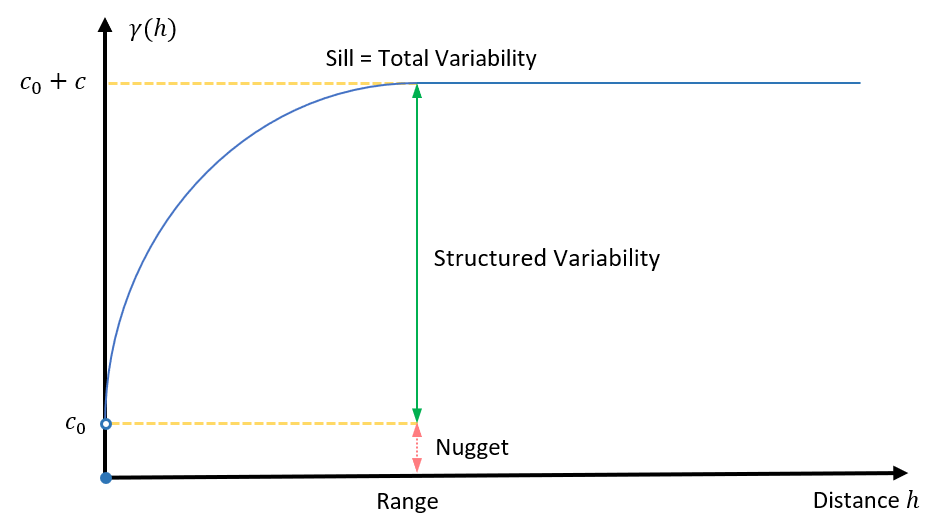
\includegraphics[width=0.75\linewidth]{nugget.png}
	\caption{A variogram plot}
\end{figure}

\paragraph{Definition 1.9} (Empirical Variogram). Suppose that we have observations $z(s_1),\cdots,z(s_n)$, an empirical semivariogram is given by
\begin{equation*}
	\hat{\gamma}(h) = \frac{1}{2\vert\mathcal{N}(h)\vert}\sum_{(i,j)\in\mathcal{N}(h)}\left\lbrace z(s_i) - z(s_j)\right\rbrace^2,\tag{1.18}
\end{equation*}
where $\mathcal{N}(h)$ is a set of observation pairs whose distance is close to $h$.

\newpage

\section{Kernel Functions}
\subsection{Inner Product and Hilbert Space}
\paragraph{Definition 2.1} (Inner product space). Let $\mathcal{H}$ be a vector space over $\mathbb{R}$. A function $\langle\cdot,\cdot\rangle_\mathcal{H}:\mathcal{H}\times\mathcal{H}\to\mathbb{R}$ is said to be an inner product on $\mathcal{H}$ if it satisfies the follwing three properties:
\begin{itemize}
	\item (Non-negativeness) $\langle f,f\rangle_\mathcal{H} \geq 0\ \forall f\in\mathcal{H}$, and $\langle f,f\rangle_\mathcal{H}=0$ if and only if $f=0$,
	\item (Symmetry) $\langle f,g\rangle_\mathcal{H} = \langle g, f\rangle_\mathcal{H},\ f,g\in\mathcal{H}$, and
	\item (Linearity) $\langle \alpha f_1 + \beta f_2,g\rangle_\mathcal{H} = \alpha\langle f_1,g\rangle_\mathcal{H} + \beta\langle f_2,g\rangle_\mathcal{H},\ \alpha,\beta\in\mathbb{R},\ f_1,f_2,g\in\mathcal{H}.$
\end{itemize}
$\mathcal{H}$ is called an inner product space. A norm is induced by the inner product: $\Vert f\Vert_\mathcal{H} = \sqrt{\langle f,f\rangle_\mathcal{H}}$.

\paragraph{Remark.} An inner product space is also called a pre-Hilbert space. Moreover, For a vector space over $\mathbb{C}$, the second property is modified as conjugate symmetry: $\langle f,g\rangle_\mathcal{H} = \overline{\langle g, f\rangle_\mathcal{H}},\ f,g\in\mathcal{H}.$

\paragraph{Definition 2.2} (Hilbert Space). A Hilbert space is a complete inner product space. In particular, every Hilbert space is a Banach space with respect to the norm induced by its inner product.

\paragraph{Remark.} Recall the definition of Cauchy sequence and Banach space:
\begin{itemize}
	\item A sequence $\lbrace f_n\rbrace_{n\in\mathbb{N}^*}\subset\mathcal{H}$ is called a Cauchy sequence with respect to norm $\Vert\cdot\Vert_\mathcal{H},$ if $\forall \varepsilon > 0,\ \exists N\in\mathbb{N}^{*}$ such that $\forall m,n > N,\ \Vert f_n - f_m\Vert_\mathcal{H}\leq\varepsilon$.
	\item A normed vector space $(\mathcal{H},\Vert\cdot\Vert_\mathcal{H})$ is called a Banach space if any Cauchy sequence $\lbrace f_n\rbrace_{n\in\mathbb{N}^*}\subset\mathcal{H}$ converges to some $f_\infty\in\mathcal{H}$, i.e. $\lim_{n\to\infty}\Vert f_n - f_\infty\Vert_\mathcal{H}=0.$
\end{itemize} 
Then, the completeness of a Hilbert space $\mathcal{H}$ states that every Cauchy sequence in $\mathcal{H}$ converges with respect to $\Vert\cdot\Vert_\mathcal{H}$ to an element in $\mathcal{H}$. 

\subsection{Kernel Functions}
\paragraph{Definition 2.3} (Kernel). Let $\mathcal{X}$ be a non-empty set. A function $k:\mathcal{X}\times\mathcal{X}\to\mathbb{R}$ is called a kernel on $\mathcal{X}$ if there exists an $\mathbb{R}$-Hilbert space $\mathcal{H}$ and a map $\phi:\mathcal{X}\to\mathcal{H}$ such that $\forall x,y\in\mathcal{X},$
\begin{equation*}
	k(x,y) = \langle\phi(x),\phi(y)\rangle_\mathcal{H}.\tag{2.1}
\end{equation*}
It is evident that $k(\cdot,\cdot)$ is symmetric, i.e. $k(x,y)=k(y,x)\ \forall,x,y\in\mathcal{X}$.
\paragraph{Remark.} In machine learning, $\phi$ is called a feature map, and $\mathcal{H}$ is called a feature space of $k$.

\paragraph{Proposition 2.4.} All kernel functions are positive definite. More specifically, let $\mathcal{X}$ be a non-empty set and $k:\mathcal{X}\times\mathcal{X}\to\mathbb{R}$ a kernel on it, then $\forall n\in\mathbb{N},\ \alpha_1,\cdots,\alpha_n\in\mathbb{R},\ x_1,\cdots,x_n\in\mathcal{X},$
\begin{equation*}
	\sum_{i=1}^n\sum_{j=1}^n \alpha_i k(x_i,x_j)\alpha_j\geq 0.\tag{2.2}
\end{equation*}

\begin{proof}
Fix $\alpha_{1:n}$ and $x_{1:n}$. Since $k(\cdot,\cdot)$ is a kernel on $\mathcal{X}$, there exists an $\mathbb{R}$-Hilbert space $\mathcal{H}$ and a map $\phi:\mathcal{X}\to\mathcal{H}$,
\begin{align*}\sum_{i=1}^n\sum_{j=1}^n \alpha_i k(x_i,x_j)\alpha_j &= \sum_{i=1}^n\sum_{j=1}^n \langle\alpha_i\phi(x_i), \alpha_j\phi(x_j)\rangle_\mathcal{H} \\
&= \left\langle\sum_{i=1}^n\alpha_i\phi(x_i), \sum_{j=1}^n\alpha_j\phi(x_j)\right\rangle_\mathcal{H} = \left\Vert\sum_{i=1}^n\alpha_i\phi(x_i)\right\Vert_\mathcal{H}^2\geq 0.\tag{2.3}
\end{align*}
Then we complete the proof.
\end{proof}

\paragraph{Theorem 2.5} (Symmetric, positive definite functions are kernels). A function $k: \mathcal{X}\times\mathcal{X}\to\mathbb{R}$ is a kernel if and only if it is symmetric and positive definite.

\begin{proof}
In view of the discussion above, it suffices to show that a symmetric and positive function $k(\cdot,\cdot)$ is a kernel. Let
\begin{equation*}
	\mathcal{H}_0 = \left\lbrace\sum_{i=1}^n x_ik(\cdot,x_i):\ n\in\mathbb{N},\ c_1,\cdots,c_n\in\mathbb{R},\ x_1,\cdots,x_n\in\mathcal{X}\right\rbrace,\tag{2.4}
\end{equation*}
and define $\langle\cdot,\cdot\rangle_{\mathcal{H}_0}: \mathcal{H}\times\mathcal{H}\to\mathbb{R}$ such that for 
\begin{align*}
	f:=\sum_{i=1}^m\alpha_ik(\cdot, x_i) \in\mathcal{H}_0,\ g:=&\sum_ {j=1}^n\beta_jk(\cdot, y_j)\in\mathcal{H}_0,\ \ x_1,\cdots,x_m,y_1,\cdots,y_n\in\mathcal{X},\tag{2.5}\\
	\langle f,g\rangle_{\mathcal{H}_0}&=\sum_{i=1}^m\sum_ {j=1}^n\alpha_i\beta_jk(x_i, y_j).\tag{2.6}
\end{align*}
You can verify that $\langle\cdot,\cdot\rangle_{\mathcal{H}_0}$ is an inner product on $\mathcal{H}_ 0$. Now let $\mathcal{H}$ be a completion of $\mathcal{H_ 0}$ with respect to $\langle\cdot,\cdot\rangle_{\mathcal{H}_ 0}$, then we have
\begin{align*}
	\langle k(\cdot, x), k(\cdot,y)\rangle_{\mathcal{H}} = \langle k(\cdot, x), k(\cdot,y)\rangle_{\mathcal{H}_0} = k(x,y)\ \forall x,y\in\mathcal{X}.\tag{2.7}
\end{align*}
Hence $\phi:x\mapsto k(\cdot,x)$ defines a feature map of $k$.
\end{proof}

\subsection{Properties of Kernels}
\paragraph{Proposition 2.6.} The linear combination, limit and pointwise product of kernels are kernels.
\begin{itemize}
	\item (Linearity) If $k_1,k_2$ are kernels, then $\forall \alpha,\beta \geq 0$, $\alpha k_1 + \beta k_2$ is a kernel.
	\item (Limit) For any kernel series $\lbrace k_n\rbrace_{n\in\mathbb{N}^{*}}$, if $\lim_{n\to\infty} k_n = k$ uniformly, then $k$ is a kernel.
	\item (Pointwise product) If $k_1,k_2$ are kernels, then $k_1\cdot k_2$ is a kernel.
\end{itemize}
\begin{proof}
We only show the third property. This is an immediate corollary of Schur's product theorem. Fix a positive integer $n$ and $\ x_1,\cdots,x_n\in\mathcal{X}$, and denote matrices
\begin{align*}
	\mathbf{K}_l = \lbrace k_l(x_i,x_j)\rbrace_{i,j=1}^n,\ l=1,2.\tag{2.8}
\end{align*}
It suffices to show the Hadamard product $\mathbf{K} = \mathbf{K_1}\circ\mathbf{K_2}$ is positive semidefinite. For any $\mathbf{a}\in\mathbb{R}^n$, denote $\mathbf{A}$ to be the diagonal matrix such that $\mathbf{A}_{ii}=\mathbf{a}_i$, then
\begin{align*}
	\mathbf{a}^\top\mathbf{Ka} &= \mathrm{trace}\left\lbrace(\mathbf{A}\mathbf{K}_1)^\top\mathbf{K}_2\mathbf{A}\right\rbrace \\
	&= \mathrm{trace}\left\lbrace\mathbf{K}_1\mathbf{A}\mathbf{K}_2\mathbf{A}\right\rbrace \\ 
	&= \mathrm{trace}\left\lbrace\mathbf{K}_1^{1/2}\mathbf{A}\mathbf{K}_2^{1/2}\mathbf{K}_2^{1/2}\mathbf{A}\mathbf{K}_1^{1/2}\right\rbrace \\
	&= \left\Vert\mathbf{K}_2^{1/2}\mathbf{A}\mathbf{K}_1^{1/2}\right\Vert_\mathrm{F}^2 \geq 0,\tag{2.9}
\end{align*}
which concludes the proof.
\end{proof}
Below are some immediate corollaries of Proposition 2.6.
\paragraph{Corollary 2.7} (Polynomial kernels). Let $\mathbf{x},\mathbf{y}\in\mathbb{R}^d$ for $d\geq 1$, and let $m$ be a positive integer and $c\geq 0$ be a non-negative real. Then
\begin{equation*}
	k(\mathbf{x},\mathbf{y}):= (c+\langle \mathbf{x},\mathbf{y}\rangle)^m\tag{2.10}
\end{equation*}
is a valid kernel.
\paragraph{Corollary 2.8} (Taylor series). Assume the Taylor series
\begin{align*}
	f(z) = \sum_{n=0}^\infty a_nz^n,\ \ \vert z\vert < r, z\in\mathbb{R}\tag{2.11}
\end{align*}
converges for some $r\in(0,\infty]$, with $a_n\geq 0$ for all $n\geq 0$. Define $\mathcal{X}$ to be the $\sqrt{r}$-ball in $\mathbb{R}^d$. Then
\begin{align*}
	k(\mathbf{x},\mathbf{y}) = f(\langle \mathbf{x}, \mathbf{y}\rangle) = \sum_{n=0}^\infty a_n\langle \mathbf{x}, \mathbf{y}\rangle^n,\  \mathbf{x},\mathbf{y}\in\mathcal{X}\tag{2.12}
\end{align*}
defines a valid kernel.

\paragraph{Corollary 2.9} (Exponential). The exponential kernel on $\mathbb{R}^d$ is defined as
\begin{align*}
k(\mathbf{x},\mathbf{y}) := \exp(\langle \mathbf{x}, \mathbf{y}\rangle),\ \mathbf{x},\mathbf{y}\in\mathbb{R}^d,\tag{2.13}
\end{align*}
and this is a valid kernel.

\subsection{Exapmles of Kernels}
\paragraph{Definition 2.10} (Gaussian RBF [radial basis function] kernels). Given $\sigma > 0$, for $\mathbf{x},\mathbf{y}\in\mathbb{R}^d$, the Gaussian RBF kernel is defined as
\begin{align*}
	k(\mathbf{x}, \mathbf{y}) = \exp\left(-\frac{1}{2\sigma^2}\Vert \mathbf{x} - \mathbf{y}\Vert^2\right).\tag{2.14}
\end{align*}
Now we are going to show that (2.14) is a valid kernel:
\begin{proof}
Let $Z$ be a $d$-dimensional Gaussian vector such that $Z\sim N(0,\sigma^{-2}I_d)$. Then the characteristic function of $Z$ can be calculated:
\begin{align*}
	\varphi_Z(\lambda) = \mathbb{E}\left[\exp\left(\mathrm{i}\lambda^\top Z\right)\right] = \exp\left(-\frac{\lambda^\top\lambda}{2\sigma^2}\right),\ \ \mathrm{i}=\sqrt{-1}.\tag{2.15}
\end{align*}
Fix $n\in\mathbb{N}^{*}$ and $\alpha_1,\cdots,\alpha_n\in\mathbb{R},\ \mathbf{x}_1,\cdots,\mathbf{x}_n\in\mathbb{R}^d$, we have
\begin{align*}
\sum_{s=1}^n\sum_{t=1}^n \alpha_s \exp\left(-\frac{\Vert \mathrm{x}_s - \mathrm{x}_t\Vert^2}{2\sigma^2}\right)\alpha_t &= \sum_{s=1}^n\sum_{t=1}^n \alpha_s\mathbb{E}\left[\exp(\mathrm{i}\mathbf{x}_s^\top Z - \mathrm{i}\mathbf{x}_t^\top Z)\right]\alpha_t \\
&= \mathbb{E} \left[\sum_{s=1}^n\sum_{t=1}^n\alpha_s\exp(\mathrm{i}\mathbf{x}_s^\top Z)  \exp(-\mathrm{i}\mathbf{x}_t^\top Z)\alpha_t\right] \\
&= \mathbb{E}\left[\sum_{s=1}^n\alpha_s\exp(\mathrm{i}\mathbf{x}_s^\top Z)  \sum_{t=1}^n\alpha_t\exp(-\mathrm{i}\mathbf{x}_t^\top Z)\right] \\
&= \mathbb{E}\left[\sum_{s=1}^n\alpha_s\exp(\mathrm{i}\mathbf{x}_s^\top Z)  \cdot\sum_{t=1}^n\alpha_t\overline{\exp(\mathrm{i}\mathbf{x}_t^\top Z)}\right] \\
&= \mathbb{E}\left[\left\vert\sum_{s=1}^n\alpha_s\exp(\mathrm{i}\mathbf{x}_s^\top Z)\right\vert^2\right] \geq 0.\tag{2.16}
\end{align*}
Therefore the Gaussian RBF is positive definite, hence is a valid kernel.
\end{proof}

\paragraph{Definition 2.11} (Laplacian kernels). Given $\alpha > 0$, for $\mathbf{x},\mathbf{y}\in\mathbb{R}^d$, the Laplacian kernel is defined as
\begin{equation*}
	k(\mathbf{x}, \mathbf{y}) = \exp\left(-\alpha\sum_{i=1}^n \vert \mathbf{x}_i - \mathbf{y}_i\vert\right).\tag{2.17}
\end{equation*}
The proof of validity is analogous to Gaussian RBF, with the Gaussian random variable replaced by Cauchy variable. Note the characteristic function of Cauchy distribution with location parameter $0$ and scale parameter $\alpha$ is $\hat{\mu}(\lambda) = \exp\left(-\alpha\vert\lambda\vert\right)$.

\paragraph{Definition 2.12} (Matérn kernels). The form of the Matérn class of functions is given by
\begin{equation*}
	k(x,y) = \frac{2^{1-\nu}}{\Gamma(\nu)}\left(\frac{\sqrt{2\nu}\vert x-y\vert}{\ell}\right)^\nu K_\nu\left(\frac{\sqrt{2\nu}\vert x-y\vert}{\ell}\right),\tag{2.18}
\end{equation*}
where $\ell > 0$ is a length-scale parameter, $\nu > 0$ is a smoothing parameter, and $K_\nu$ is the modified Bessel function of second type.

\paragraph{Remark.} In equation (2.18), the parameter $\nu$ controls the smoothness of our kernel, and $\ell$ is the band width.

\newpage

\section{Gaussian Process}
\subsection{Definition and properties}
The Gaussian process can be seen as an extension of multivariate Gaussian distribution from finite-dimensional case to infinite-dimensional case. It is a stochastic process or a random field (a collection of random variables indexed by time or space) such that the joint distribution of every finite collection of those random variables is Gaussian.
\paragraph{Definition 3.1} (Gaussian process). Given a probability space $(\Omega,\mathcal{F},\mathbb{P})$ and an index set $\mathcal{D},$ a random field $\left\lbrace Z(s)\in L_2(\Omega):\ s\in\mathcal{D}\right\rbrace$ is called a Gaussian process, if for every finite set of indices $\lbrace s_1,\cdots,s_n\rbrace \subset \mathcal{D},$ the joint distribution of random variables $Z(s_1),\cdots,Z(s_n)$ is a multivariate Gaussian distribution.

The mean and covariance function of a Gaussian process is defined by
\begin{align*}
	\mu(s):=\mathbb{E}[Z(s)],\ k(s,t):=\mathrm{Cov}\left\lbrace Z(s),z(t)\right\rbrace,\tag{3.1}
\end{align*}
and they completely determine a Gaussian process $\mathcal{GP}\left(\mu(\cdot),k(\cdot,\cdot)\right).$

\paragraph{Properties of Gaussian processes}
\begin{itemize}
\item A Gaussian process can be seen as a distribution over real-valued functions $\lbrace f:\mathcal{D}\to\mathbb{R}\rbrace.$ Suppose that $f\sim\mathcal{GP}\left(\mu(\cdot),k(\cdot,\cdot)\right),$ then $\forall n\in\mathbb{N}^*,\ x_1,\cdots,x_n\in\mathcal{D},$ the joint distribution of $f(x_1),\cdots,f(x_n)$ is given by
\begin{equation*}
	\begin{pmatrix} f(x_1) \\ \vdots\\ f(x_n) \end{pmatrix} \sim N\left\lbrace
	\begin{pmatrix} \mu(x_1) \\ \vdots\\ \mu(x_n) \end{pmatrix},
	\begin{pmatrix} k(x_1,x_1) & \cdots & k(x_1,x_n) \\ \vdots & \ddots & \vdots\\ k(x_n, x_1) & \cdots & k(x_n,x_n) \end{pmatrix}\right\rbrace.\tag{3.2}
\end{equation*}
\item The covariance function $k$ is a kernel which is symmetric and positive definite. A wide range of kernels can be selected as the covariance function, such as Gaussian RBF and Matérn kernels.
\item If a Gaussian process $Z(\cdot)$ is (weakly) stationary, i.e. it has constant mean $\mu$, and the covariance $k(s,t)$ depends on only the difference between locations $s-t$, then $\forall n\in\mathbb{N}^*,\ s_1,\cdots,s_n\in\mathcal{D},$ and $\forall h$ such that $s_1+h,\cdots,s_n+h\in\mathcal{D}$, then
\begin{align*}
	\left(Z(s_1),\cdots,Z(s_n)\right) \overset{d}{=} \left(Z(s_1 + h),\cdots,Z(s_n + h)\right).\tag{3.3}
\end{align*}
In a nutshell, weak stationarity implies strict stationarity in Gaussian processes.
\end{itemize}

\paragraph{} Some Gaussian processes with zero mean and different covariance kernels are visualized below.
\begin{figure}[H]
	\centering
	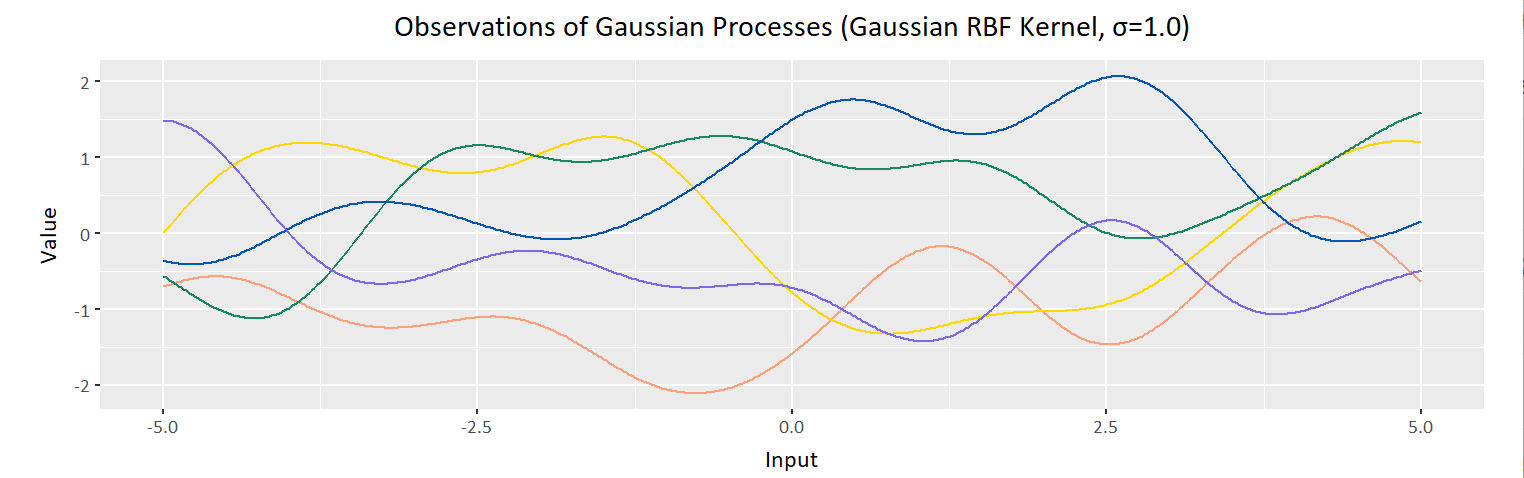
\includegraphics[width=0.8\linewidth]{rbf.png}
	\caption{Sample paths of Gaussian processes with Gaussian RBF kernel as its covariance}
\end{figure}
\begin{figure}[H]
	\centering
	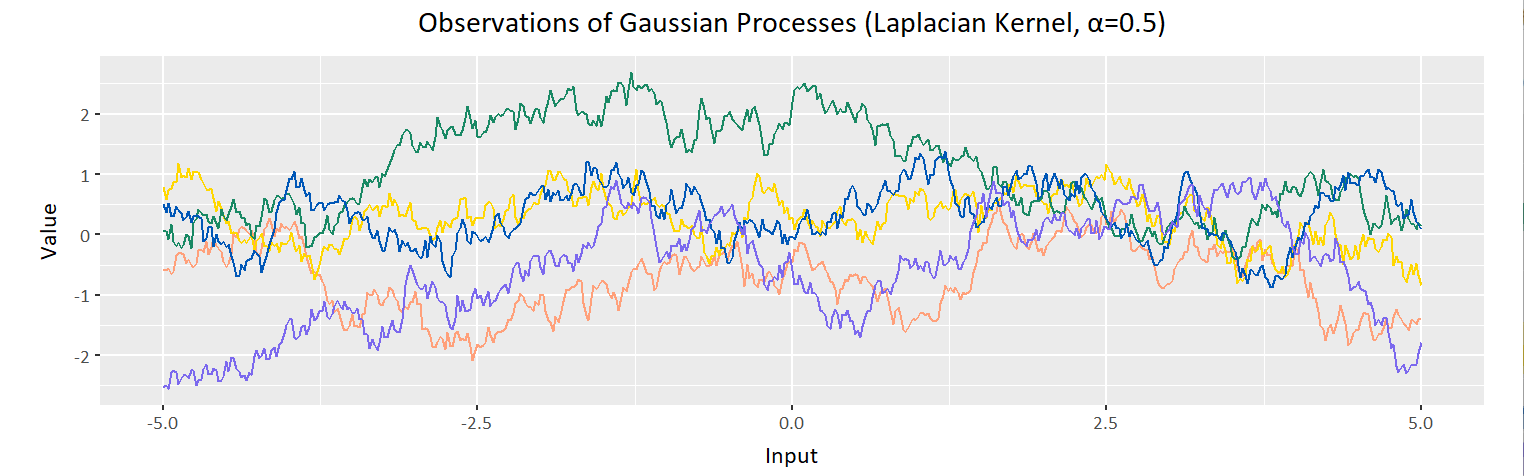
\includegraphics[width=0.8\linewidth]{lap.png}
	\caption{Sample paths of Gaussian processes with Laplacian RBF kernel as its covariance}
\end{figure}

\subsection{Hierarchical model for geostatistical process}
In practice, we often apply a hierarchical model to simulate spatial or geostatistical data. A hierarchical model has two components: a process model, which sets up some latent variable with covariance structure, and a data model, which generates observations from latent variables with measurement error.

\paragraph{Process Model.} Suppose that $\mathbf{m}(\cdot)\in\mathbb{R}^p$ is a column vector of covariates related to the mean function. Given regression coefficients $\beta\in\mathbb{R}^p$ and kernel $k(\cdot,\cdot),$ let
\begin{align*}
	Z(\cdot)\sim\mathcal{GP}\left(\mathbf{m}(\cdot)^\top\beta, k(\cdot,\cdot)\right).\tag{3.4}
\end{align*}
\paragraph{Data Model.} Conditioning on process $Z(\cdot),$ the observation at location $s\in\mathcal{D}$ is
\begin{align*}
	Y(s)|Z(\cdot) \sim N(Z(s), \sigma^2),\ \sigma^2>0;\tag{3.5}
\end{align*}
Equivalently, for $n$ locations $s_1,\cdots,s_n,$
\begin{align*}
	Y(s_i) = Z(s_i) + e_i,\ e_i \overset{\textrm{i.i.d.}}{\sim} N(0,\sigma^2),\ i=1,\cdots,n. \tag{3.6}
\end{align*}
Hence we can use an error process $\epsilon(\cdot)$ to model our observational data:
\begin{align*}
	Y(s_i) = \mathbf{m}(s_i)^\top\beta + \epsilon(s_i),\ \begin{pmatrix}\epsilon(s_1)\\ \vdots \\ \epsilon(s_n)\end{pmatrix}\sim N(0,\mathbf{K} + \sigma^2\mathbf{I}_n),\tag{3.7}
\end{align*}
where $\mathbf{K} = \lbrace k(s_i,s_j)\rbrace_{i,j=1}^n.$

\subsection{Analytical Examples}
\subsubsection{Brownian Motion}
\paragraph{Definition 3.2} (Brownian motion/Wiener process). Given a probability space $(\Omega,\mathcal{F},\mathbb{R}),$ a stochastic process $\lbrace W(t): \Omega\to\mathbb{R},\ t\geq 0\rbrace$ is called a \textit{Brownian motion}, if it satisfies the following:
\begin{itemize}
	\vspace{0.1cm}
	\item $\mathbb{P}\lbrace W(0) = 0\rbrace = 1;$
	\vspace{0.1cm}
	\item The sample paths of $W(t)$ are continuous;
	\vspace{0.1cm}
	\item $W(t)$ has independent and stationary increments;
	\vspace{0.1cm}
	\item $W(t)\sim N(0,\sigma^2t),\ \sigma > 0.$
\end{itemize}
For convenience of our discussion, we will consider standard Brownian motion in which $\sigma^2=1.$ Let $W(\cdot)$ be a standard Brownian motion, let's investigate the properties of $W(\cdot).$

\paragraph{Proposition 3.3} (Mean and Covariance). $\mathbb{E}[W(t)] = 0,\ \mathrm{Cov}\lbrace W(s),W(t)\rbrace = \min(s,t).$
\begin{proof}
The mean of $W(t)$ is zero by definition, so we only consider the covariance. Without loss of generality, suppose $s<t$ (the case $s = t$ is trivial). Note that $W(t)$ has independent increments, we have
\begin{equation*}
	W(s)\perp W(t) - W(s),\ \mathbb{E}\left[W(s)\left(W(t)-W(s)\right)\right] = 0.\tag{3.8}
\end{equation*}
Hence
\begin{align*}
	\mathrm{Cov}\lbrace W(s),W(t)\rbrace &= \mathbb{E}[W(s)W(t)]\\
	&= \mathbb{E}[W(s)^2] + \mathbb{E}[W(s)(W(t)-W(s))] = s,\tag{3.9}
\end{align*}
which concludes the proof.
\end{proof}

\paragraph{Proposition 3.4} (Gaussianity). $W(\cdot)$ is a Gaussian process with zero mean and kernel $k(s,t):=\min(s,t).$
\begin{proof}
It suffices to show that $\forall n\geq 1,\ 0 < t_1 < \cdots < t_n,$ the joint distribution of corresponding variables $\mathbf{W} = (W(t_1),\cdots,W(t_n))^\top$ is Gaussian. Denote Brownian increments
\begin{align*}
	\mathbf{Z}=\left(W(t_1),W(t_2)-W(t_1),\cdots,W(t_n) - W(t_{n-1})\right)^\top,\tag{3.10}
\end{align*}
By stationarity and independence of increments, we have $\mathbf{Z}\sim N(0,\mathbf{D})$, where $\mathbf{D} = \mathrm{diag}\lbrace t_1, t_2-t_1,\cdots,t_n-t_{n-1}\rbrace.$ Denote lower triangular matrix
\begin{align*}
	\mathbf{L} = \left\lbrace\mathbbm{1}_{\{i\geq j\}}\right\rbrace_{i,j=1}^n = 
	\begin{pmatrix} 1 & 0 & \cdots & 0 & 0 \\
		1 & 1 & \cdots & 0 & 0\\
		\vdots & \vdots & \ddots & \vdots & \vdots\\
		1 & 1 & \cdots & 1 & 0\\
		1 & 1 & \cdots & 1 & 1\end{pmatrix},\tag{3.11}
\end{align*}
\begin{align*}
	\mathbf{LZ} \sim N(0,\mathbf{LDL}^\top)\ \Rightarrow\ \mathbf{W}\sim N(0,\mathbf{K}),\tag{3.12}
\end{align*}
where $\mathbf{K}=\left\lbrace \min(t_i,t_j)\right\rbrace_{i,j=1}^n.$ Hence $\mathbf{W}$ is Gaussian, and $W(t)$ is a Gaussian process.
\end{proof} 


\subsubsection{Ornstein–Uhlenbeck process (O-U process)}
Given a probability space $(\Omega,\mathcal{F},\mathbb{R})$ and a Brownian motion $W(\cdot)$ defined on this space, An Ornstein–Uhlenbeck process $\lbrace X(t): \Omega\to\mathbb{R},\ t\geq 0\rbrace$ is defined by the following stochastic differential equation (SDE):
\begin{align*}
	\mathrm{d}X(t) = -\theta X(t)\mathrm{d}t + \sigma\mathrm{d}W(t),\tag{3.13}
\end{align*}
where $\theta>0$ and $\sigma>0$. Let's derive the solution of the SDE above:
\begin{align*}\mathrm{d}X(t)  + \theta X(t)\mathrm{d}t &= \sigma\mathrm{d}W(t),\\
\mathrm{d}\left(X(t)\mathrm{e}^{\theta t}\right) &= \sigma\mathrm{e}^{\theta t}\mathrm{d}W(t),\\
X(t)\mathrm{e}^{\theta t} - X(0) &= \sigma\int_0^t\mathrm{e}^{\theta s}\mathrm{d}W(s).\tag{3.14}
\end{align*}
So analytical form of $X(t)$ is
\begin{align*}
	X(t) = X(0)\mathrm{e}^{-\theta t} + \sigma\int_0^t\mathrm{e}^{-\theta(t-s)}\mathrm{d}W(s).\tag{3.15}
\end{align*}
Now we are going to investigate the properties of Ornstein-Uhlenbeck process.

\paragraph{Proposition 3.4} Let $X(\cdot)$ be an Ornstein–Uhlenbeck process defined above. Conditional on $X(0),$ the mean and variance of $X(\cdot)$ is given by
\begin{align*}
	\mathbb{E}[X(t)|X(0)] &= X(0)\mathrm{e}^{-\theta t},\\
	\mathrm{Cov}\left\lbrace X(s), X(t)|X(0)\right\rbrace &= \frac{\sigma^2}{2\theta}\left(\mathrm{e}^{\theta\vert t-s\vert} - \mathrm{e}^{-\theta(s+t)}\right).\tag{3.16}
\end{align*}
\begin{proof}
The conditional expectation of $X(t)$ is its deterministic part, since the stochastic part is an integral of Brownian increments with zero mean. It remains to derive the covariace.
\begin{align*}
	\mathrm{Cov}\left\lbrace X(s), X(t)|X(0)\right\rbrace = \sigma^2\mathrm{e}^{-(s+t)}\mathbb{E}\left[\int_0^s \mathrm{e}^{\theta u}\mathrm{d}W(u)\int_0^t \mathrm{e}^{\theta u}\mathrm{d}W(u)\right].\tag{3.17}
\end{align*}
By the independence of Brownian increments and the Itô isometry, we have
\begin{align*}\mathbb{E}\left[\int_0^s \mathrm{e}^{\theta u}\mathrm{d}W(u)\int_0^t \mathrm{e}^{\theta u}\mathrm{d}W(u)\right] &= \mathbb{E}\left[\left(\int_0^{\min(s,t)} \mathrm{e}^{\theta u}\mathrm{d}W(u)\right)^2\right]\\
&= \int_0^{\min(s,t)} \mathrm{e}^{2\theta u}\mathrm{d}u = \frac{1}{2\theta}\left(\mathrm{e}^{2\theta\min(s,t)} - 1\right).\tag{3.18}
\end{align*}
Therefore
\begin{align*}
	\mathrm{Cov}\left\lbrace X(s), X(t)|X(0)\right\rbrace = \frac{\sigma^2}{2\theta}\left(\mathrm{e}^{-\theta\vert t-s\vert} - \mathrm{e}^{-\theta(t+s)}\right),\tag{3.19}
\end{align*}
and we complete the proof.
\end{proof} 
\paragraph{Proposition 3.5} (Gaussianity). We impose a Gaussian distribution $N(0,\frac{\sigma^2}{2\theta})$ on $X(0)$ which is independent of $W(\cdot),$ then
\begin{align*}
	\mathbb{E}[X(t)] = 0,\quad
	\mathrm{Cov}\left\lbrace X(s), X(t)\right\rbrace = \frac{\sigma^2}{2\theta}\mathrm{e}^{\theta\vert t-s\vert},\tag{3.20}
\end{align*}
which implies that an (unconditioned) Ornstein–Uhlenbeck process is a stationary Gaussian process with zero mean and absolute exponential kernel.
\begin{proof}
Since $X(0)$ is independent of $W(\cdot)$, we only need to add the term $\mathrm{e}^{-\theta(s+t)}\mathrm{Var}(Z_0)$ to the conditional covariance. To show that the Ornstein–Uhlenbeck process is a Gaussian process, it remains to consider the stochastic part of $X(t):$
\begin{align*}
	\int_0^t\mathrm{e}^{-\theta(t-s)}\mathrm{d}W(s) = \lim_{n \to \infty}\sum_{[t_{i-1},t_i]\in \pi_n}\mathrm{e}^{-\theta(t-s_{i-1})}\left(W(s_i) - W(s_{i-1})\right),\tag{3.21}
\end{align*}
where $\lbrace\pi_n\rbrace$ is a sequence of partitions of $[0,t]$ with the length of maximum sub-interval going to zero. Since all Brownian increments $W(s_i) - W(s_{i-1})$ are Gaussian,  the linear combination of finite Brownian increments is Gaussian. Furthermore, the Itô integral as the $L^2$-limit of a sequence of Gaussian variables is still Gaussian. Hence $X(\cdot)$ is a Gaussian process.
\end{proof}

\paragraph{Remark.} A more general form of Ornstein–Uhlenbeck processes has an additional drift term $\mu$:
\begin{align*}
	\mathrm{d}X(t) = \theta (\mu -X(t))\mathrm{d}t + \sigma\mathrm{d}W(t).\tag{3.22}
\end{align*}
The drift term does not change the form of covariance, but the conditional mean need to be modified:
\begin{equation*}
	\mathbb{E}[X(t)\vert X(0)] = X(0)\mathrm{e}^{-\theta t} + \mu(1-\mathrm{e}^{-\theta t}).\tag{3.23}
\end{equation*}

\newpage

\section{Kriging}
\paragraph{Nomenclature.} Kriging is a method of interpolation based on Gaussian process, and is also known as Gaussian process regression (GPR). Georges Matheron established the theoretic basis of this spatial interpolation technique in 1960, and named it kriging (\textit{French: krigeage}) to honor the pioneering work of Danie G. Krige in geostatistics.

Given a random field $\lbrace Z(s): s\in\mathcal{D}\rbrace$ with its observation at location $s_1,\cdots,s_n,$ the goal of kriging is to predict $Z(\cdot)$ at an arbitrary location $s\in\mathcal{D}.$

\subsection{Simple Kriging}
In simple kriging, the mean of spatial field is known. Without loss of generality, set it to be zero. Let $f:\mathcal{X}\to{\mathbb{R}}$ be the field of interest and $f\sim\mathcal{GP}\left(0,k(\cdot,\cdot)\right),$ we will interpolate the value of $f$ at an arbitrary location using its finite observations. Please note that $f$ is not a random field or a Gaussian process itself since it is deterministic. Instead, $f$ is a realization of the aforementioned Gaussian process. In the context of Bayesian regression, $\mathcal{GP}(0,k(\cdot,\cdot))$ is the prior distribution of $f$.

We first introduce some notations. Given locations $x_1,\cdots,x_N\in\mathcal{X},$ we use $\mathbf{K}$ to denote the covariance matrix of $\left(f(x_1),\cdots,f(x_N)\right)^\top,$ i.e., $\mathbf{K} = \lbrace k(x_i,x_j)\rbrace_{i,j=1}^N\in\mathbb{R}^{n\times n}$. We define $\mathbf{k}(\cdot): \mathcal{X}\to\mathbf{R}^N$ to be such that
\begin{equation*}
	\mathbf{k}(x) = \left(k(x,x_1),\cdots,k(x,x_N)\right)^\top.\tag{4.1}
\end{equation*}

\subsubsection{Noise-free observations}
We suppose that our observations are faithful, that is, the observation at location $x_i$ is the true value of $f(x_i)$. If we have observations at $N$ distinct locations $x_1,\cdots,x_N\in\mathcal{X},$ then our dataset is $\left\lbrace\left(x_i,f(x_i)\right)\right\rbrace_{i=1}^N.$ Denote $\mathbf{f} = \left(f(x_1),\cdots,f(x_N)\right)^\top,$ the posterior of $f$ at any location is given by the following theorem.

\paragraph{Theorem 4.1} (Posterior of $f$ conditioning on noise-free observations). Under the notations above plus $\mathbf{K}$ is nonsingular, the posterior of $f$ at an arbitrary location $x\in\mathcal{X}$ is Gaussian. The mean and variance is given by
\begin{align*}
	\mathbb{E}\left[f(x)|\mathbf{f}\,\right] &= \mathbf{k}(x)^\top\mathbf{K}^{-1} \mathbf{f},\tag{4.2}\\
	\mathrm{Var}\left\lbrace f(x)|\mathbf{f}\,\right\rbrace &= k(x,x) - \mathbf{k}(x)^\top\mathbf{K}^{-1}\mathbf{k}(x).\tag{4.3}
\end{align*}
Moreover, $\forall x,x'\in\mathcal{X}$,
\begin{align*}
	\mathrm{Cov}\left\lbrace f(x), f(x')|\mathbf{f}\,\right\rbrace = k(x,x') - \mathbf{k}(x)^\top\mathbf{K}^{-1} \mathbf{k}(x').\tag{4.4}
\end{align*}
\begin{proof}
$\forall x,x'\in\mathcal{X}$, the joint distribution of $\left(f(x),f(x'),f(x_1),\cdots,f(x_n)\right)^\top$ can be derived:
\begin{align*}
	\begin{pmatrix} f(x) \\ f(x') \\ \mathbf{f}\end{pmatrix} \sim N\left\lbrace \mathbf{0},\begin{pmatrix}
		k(x,x) & k(x,x') & \mathbf{k}(x)^\top \\
		k(x', x) & k(x',x') & \mathbf{k}(x')^\top \\
		\mathbf{k}(x) & \mathbf{k}(x') & \mathbf{K}
	\end{pmatrix}\right\rbrace.\tag{4.5}
\end{align*}
Then conditional on $\mathbf{f},$  the distribution of $(f(x),f(x'))^\top$ is still Gaussian:
\begin{align*}
	\left.\begin{pmatrix} f(x) \\ f(x')\end{pmatrix}\right|\,\mathbf{f} \sim N\left\lbrace
	\begin{pmatrix}
		\mathbf{k}(x)^\top \\
		\mathbf{k}(x')^\top
	\end{pmatrix}\mathbf{K}^{-1}\mathbf{f},\ 
	\begin{pmatrix}
		k(x,x) & k(x,x') \\
		k(x', x) & k(x',x')
	\end{pmatrix} - \begin{pmatrix}
		\mathbf{k}(x)^\top \\
		\mathbf{k}(x')^\top
	\end{pmatrix}\mathbf{K}^{-1}\left(\mathbf{k}(x),\mathbf{k}(x')\right)\right\rbrace.\tag{4.6}
\end{align*}
Thus we complete the proof.
\end{proof} 

\paragraph{Remark.}
(I) When $x$ is some $x_i\in\lbrace x_1,\cdots, x_N\rbrace$, the posterior of $f(x_i)$ reduces to the Dirac measure centered on $\mathbf{f}_i.$ To see this, note that
\begin{align*}
	\mathbf{e}_i = \mathbf{K}^{-1}\mathbf{Ke}_i = \mathbf{K}^{-1}\mathbf{k}(x_i),\tag{4.7}
\end{align*}
then
\begin{align*}
	\mathbb{E}\left[f(x_i)|\mathbf{f}\,\right] = \mathbf{e}_i\mathbf{f} = f(x_i),\ \mathrm{Var}\left\lbrace f(x)|\mathbf{f}\,\right\rbrace = k(x_i,x_i) - \mathbf{k}(x_i)^\top\mathbf{e}_i = 0.\tag{4.8}
\end{align*}
(II) Define $\mu^\perp(x) = \mathbf{f}^\top\mathbf{K}^{-1}\mathbf{k}(x),\ k^\perp(x,x') = k(x,x') - \mathbf{k}(x)^\top\mathbf{K}^{-1} \mathbf{k}(x'),$ the posterior of $f$ is a Gaussian process:
\begin{align*}
	f\,|\,\mathbf{f} \sim\mathcal{GP}\left(\mu^\perp(\cdot),\ k^\perp(\cdot,\cdot)\right).\tag{4.9}
\end{align*}
To show this you need to verify that $k^\perp(\cdot,\cdot)$ is a valid kernel, i.e., $k^\perp(\cdot,\cdot)$ is positive definite. You may use Schur's complement to derive the form of $k^\perp(\cdot,\cdot).$

\subsubsection{Observations with additive noise}
In a real scenario, the true process $f$ is not accessible due to random fluctuation or measurement error. Like in hierarchical model, assume that there exists additive noise in our observational data:
\begin{align*}
	y_i = f(x_i) + \varepsilon_i,\ \varepsilon_i\overset{\mathrm{i.i.d.}}{\sim} N(0,\sigma^2),\tag{4.10}
\end{align*}
then the posterior of $f$ at any location need to be modified.

\paragraph{Theorem 4.2} (Posterior of $f$ conditioning on observations with additive noise). Under the notations above with observations $Y=(y_1,\cdots,y_N)^\top,$ the posterior of $f$ at an arbitrary location $x\in\mathcal{X}$ is Gaussian. The mean and variance is given by
\begin{align*}
	\mathbb{E}\left[f(x)\,|\,Y\right] &= \mathbf{k}(x)^\top\left(\mathbf{K} + \sigma^2\mathbf{I}_{N}\right)^{-1} Y,\tag{4.11}\\
	\mathrm{Var}\left\lbrace f(x)\,|\,Y\right\rbrace &= k(x,x) - \mathbf{k}(x)^\top\left(\mathbf{K} + \sigma^2\mathbf{I}_{N}\right)^{-1}{\mathbf{k}}(x).\tag{4.12}
\end{align*}
Moreover, $\forall x,x'\in\mathcal{X}$,
\begin{align*}
	\mathrm{Cov}\left\lbrace f(x), f(x')\,|\,Y\right\rbrace = k(x,x') - \mathbf{k}(x)^\top\left(\mathbf{K} + \sigma^2\mathbf{I}_{N}\right)^{-1}{\mathbf{k}}(x').\tag{4.13}
\end{align*}
\begin{proof}
Analogous to Theorem 1, use the joint distribution of $\left(f(x),f(x'),Y\right)$ to derive the conditional (posterior) distribution. 
\end{proof} 
\paragraph{Remark.} The posterior of $f$ is a Gaussian process with the mean and covariance function given by Theorem 4.2. A point estimator is the expectation:
\begin{align*}
	\hat{f}(\cdot) = Y^\top(\mathbf{K}+\sigma^2\mathbf{I}_N)^{-1}\mathbf{k}(\cdot),\tag{4.14}
\end{align*}
which is a linear combination of $\lbrace k(\cdot,x_i)\rbrace_{i=1}^N.$

\subsubsection{Overlapping observations}
In previous discussions, locations $x_1,\cdots,x_N$ are supposed to be distinct. In other words, we have only one observation for a unique location. Now we suppose that we have $N$ observations at $n$ unique locations $\bar{x}_ 1,\cdots,\bar{x}_ n$ with $n < N.$ At each location $\bar{x}_ j$, we have $a_ j$ observations $y_ {j,1},\cdots,y_ {j,a_ j},$ with $j=1,\cdots,n,\ a_1+\cdots+a_n = N$ and $\max_{1\leq j\leq n} a_j > 1$.
\paragraph{} We first introduce some notations.
\begin{align*}
	(x_1,\cdots, x_N) &= (\underbrace{\bar{x}_1,\cdots,\bar{x}_1}_{a_1},\ \underbrace{\bar{x}_2,\cdots,\bar{x}_2}_{a_2},\cdots,\underbrace{\bar{x}_n,\cdots,\bar{x}_n}_{a_n}) \in\mathcal{X}^N,\tag{4.15}\\
	Y &= (y_{1,1},\cdots,y_{1,a_1},y_{2,1},\cdots,y_{2,a_2},\cdots,y_{n,1},\cdots,y_{n,a_n})\in\mathbb{R}^N,\tag{4.16}\\
	\bar{Y} &= (\bar{y}_1,\cdots,\bar{y}_n)\in\mathbb{R}^n,\ \ \bar{y}_j = \frac{1}{a_j}\sum_{l=1}^{a_j}y_{j,a_j}.\tag{4.17}
\end{align*}

Moreover, denote
\begin{align*}
	\bar{\mathbf{k}}(x) = \left(k(x,\bar{x}_1),\cdots,k(x,\bar{x}_n)\right)^\top\in\mathbb{R}^n,\ \ \bar{\mathbf{K}} = \lbrace k(\bar{x}_i,\bar{x}_j)\rbrace_{i,j=1}^n\in\mathbb{R}^{n\times n}.\tag{4.18}
\end{align*}

Let $\mathbf{U}\in\mathbb{R}^{N\times n}$ be a block diagonal matrix such that $\mathbf{U}=\mathrm{diag}\lbrace \mathbf{1}_ {a_ 1},\cdots,\mathbf{1}_ {a_ n}\rbrace$, where $\mathbf{1}_ {a_j}$ is an $a_j$-dimensional all-one vector, and let $\mathbf{A} = \mathrm{diag}\lbrace a_1,\cdots,a_n\rbrace.$ 

\paragraph{Proposition 4.3.} With the notations above, we have \begin{align*}
	\bar{Y} = \mathbf{A}^{-1}\mathbf{U}^\top Y,\ \bar{\mathbf{k}}(x) = \mathbf{A}^{-1}\mathbf{U}^\top\mathbf{k}(x),\ \mathbf{k}(x) = \mathbf{U}\bar{\mathbf{k}}(x),\ \mathbf{K} = \mathbf{U}\bar{\mathbf{K}}\mathbf{U}^\top.\tag{4.19}
\end{align*}
These equalities can be verified by direct calculation.

\paragraph{Proposition 4.4.} Suppose $\sigma^2 > 0,$ then $\mathbf{U}^\top\left(\sigma^2\mathbf{I}_N + \mathbf{K}\right)^{-1}\mathbf{U} = \left(\sigma^2\mathbf{A}^{-1} + \bar{\mathrm{K}}\right)^{-1}.$
\begin{proof}
Recall the Sherman-Morrison-Woodbury formula:
\begin{align*}
	(\mathbf{A} + \mathbf{UCV})^{-1} = \mathbf{A}^{-1} - \mathbf{A}^{-1}\mathbf{U}\left(\mathbf{C}^{-1} + \mathrm{V}\mathbf{A}^{-1}\mathrm{U}\right)^{-1}\mathbf{V}\mathbf{A}^{-1},\tag{4.20}
\end{align*}
we have
\begin{align*}
	\left(\sigma^2\mathbf{I}_N + \mathbf{K}\right)^{-1} = \left(\sigma^2\mathbf{I}_N + \mathbf{U}\bar{\mathbf{K}}\mathbf{U}^\top\right)^{-1} = \sigma^{-2}\mathbf{I}_N - \sigma^{-4}\mathrm{U}\left(\bar{\mathbf{K}}^{-1} + \sigma^{-2}\mathbf{U}^\top\mathbf{U}\right)^{-1}\mathbf{U}^\top.\tag{4.21}
\end{align*}
Note that $\mathbf{U}^\top\mathbf{U} = \mathbf{A}$, then
\begin{align*}
	\mathbf{U}^\top\left(\sigma^2\mathbf{I}_N + \mathbf{K}\right)^{-1}\mathbf{U} = \sigma^{-2}\mathbf{A} - \sigma^{-4}\mathbf{A}\left(\bar{\mathbf{K}}^{-1} + \sigma^{-2}\mathbf{A}\right)^{-1}\mathbf{A}.\tag{4.22}
\end{align*}
Using the Sherman-Morrison-Woodbury formula, we have
\begin{align*}
	\sigma^{-2}\mathbf{A} + \sigma^{-4}\mathbf{A}\left(\bar{\mathbf{K}}^{-1} + \sigma^{-2}\mathbf{A}\right)^{-1}\mathbf{A} = \left(\sigma^2\mathbf{A}^{-1} + \bar{\mathbf{K}}\right)^{-1},\tag{4.23}
\end{align*}
which concludes the proof.
\end{proof} 

\paragraph{Theorem 4.5} (Posterior of $f$ conditioning on overlapping observations). Under the notations above, the posterior of $f$ at an arbitrary location $x\in\mathcal{X}$ is Gaussian. The mean and variance is given by
\begin{align*}\mathbb{E}\left[f(x)\,|\,\bar{Y}\right] &= \bar{\mathbf{k}}(x)^\top\left(\bar{\mathbf{K}} + \sigma^2\mathbf{A}^{-1}\right)^{-1}\bar{Y},\tag{4.24}\\
\mathrm{Var}\left\lbrace f(x)\,|\,\bar{Y}\right\rbrace &= k(x,x) - \bar{\mathbf{k}}(x)^\top\left(\bar{\mathbf{K}} + \sigma^2\mathbf{A}^{-1}\right)^{-1}\bar{\mathbf{k}}(x).\tag{4.25}
\end{align*}
Moreover, $\forall x,x'\in\mathcal{X}$,
\begin{align*}
\mathrm{Cov}\left\lbrace f(x), f(x')\,|\,\bar{Y}\right\rbrace = k(x,x') - \bar{\mathbf{k}}(x)^\top\left(\bar{\mathbf{K}} + \sigma^2\mathbf{A}^{-1}\right)^{-1}\bar{\mathbf{k}}(x').\tag{4.26}
\end{align*}
\begin{proof}
	Plug in Proposition 1 and 2 to the posterior of $f$ given in Theorem 2.
\end{proof} 

\subsection{Universal Kriging}
In universal kriging, the mean of spatial field is unknown. To apply regression, we choose a group of basis functions $\lbrace m_1(\cdot),\cdots,m_p(\cdot)\rbrace$ from $L_2(\mathcal{X})$ and denote $\mathbf{m}(\cdot) = \bigl(m_1(\cdot),\cdots,m_p(\cdot)\bigr)^\top:\mathcal{X}\to\mathbb{R}^p.$ Assume that $f\sim\mathcal{GP}\left(\mathbf{m}(\cdot)^\top\beta,\ k(\cdot,\cdot)\right),$ where $\beta\in\mathbb{R}^p$ is unknown, and that our observations $\left.Y(x)\right\vert f\sim N(f(x),\sigma^2).$ Note these assumptions implies the independence of $\left\lbrace \left.Y(x)\right\vert x\in\mathcal{X}\right\rbrace$ given $f.$ Then, we can define the error process
\begin{equation*}
	\epsilon(x) := Y(x) - \mathbf{m}(x)^\top\beta,\tag{4.27}
\end{equation*}
which implies the following distribution of observations at $x_1,\cdots,x_n$:
\begin{align*}
	\epsilon(x_{1:n})\sim N(0,\Sigma),\ \ \Sigma = \mathbf{K} + \sigma^2\mathbf{I}_n,\ \ \mathbf{K} = \lbrace k(x_i,x_j)\rbrace_{i,j=1}^n.\tag{4.28}
\end{align*}
Furthermore, the joint distribution of our observations can be induced:
\begin{align*}
	\mathbf{Y} := \left(Y(x_1),\cdots,Y(x_n)\right)^\top\sim N\left(\mathbf{M}\beta,\Sigma\right),\ \ \mathbf{M} = \left(\mathbf{m}(x_1),\cdots,\mathbf{m}(x_n)\right)^\top\in\mathbb{R}^{n\times p}.\tag{4.29}
\end{align*}
Now we derive the best unbiased linear prediction (BLUP) of $Y(x)$ for arbitrary $x\in\mathcal{X}.$ Generally, we have the following result.

\paragraph{Theorem 4.6} (Universal kriging). Suppose the covariance matrix of $\mathbf{Y}=\left(Y(x_1),\cdots,Y(x_n)\right)$ is nonsingular, and $\mathbf{M}=\left(\mathbf{m}(x_1),\cdots,\mathbf{m}(x_n)\right)^\top$ is of full column rank. Then for $x\in\mathcal{X},$ the BLUP of $Y(x)$ is given by
\begin{align*}
	\hat{Y}(x) = \mathbf{m}(x)^\top\hat{\beta} + \mathbf{k}(x)^\top\Sigma^{-1}\left(\mathbf{Y} - \mathbf{M}\hat{\beta}\right),\tag{4.30}
\end{align*}
where $\hat{\beta} = \left(\mathbf{M}^\top\Sigma^{-1}\mathbf{M}\right)^{-1}\mathbf{M}^\top\Sigma^{-1}\mathbf{Y}.$
\begin{proof}
The derivation of BLUP is straight forward but tedious. We first express the prediction of $Y(x)$ as a linear combination:
\begin{align*}
	\hat{Y}(x) = \lambda_0(x) + \sum_{i=1}^n \lambda_i(x) Y(x_i) = \lambda_0(x) + \lambda(x)^\top\mathbf{Y}.\tag{4.31}
\end{align*}
The unbiasedness of BLUP implies that
\begin{align*}
	\mathbf{m}(x)^\top\beta = \mathbb{E}\left[\hat{Y}(x)\right] = \lambda_0(x) + \lambda(x)^\top\mathbf{M}\beta\ \ \ \forall\beta\in\mathbb{R}^p.\tag{4.32}
\end{align*}
Set $\beta=0,$ we have $\lambda_0(x)=0.$ To solve the BLUP, which has the minimum variance across all predictions of the form above, one need to consider the following optimization problem:
\begin{align*}
	\min_{\lambda(x)\in\mathbb{R}^p}\ \ \mathbb{E}\left[\left(Y(x) - \lambda(x)^\top\mathbf{Y}\right)^2\right]\ \ \ \textrm{subjected to}\ \ \ \mathbf{M}^\top\lambda(x) = \mathbf{m}(x).\tag{4.33}
\end{align*}
The mean square error of BLUP is
\begin{align*}
	\mathbb{E}\left[\left(Y(x) - \lambda(x)^\top\mathbf{Y}\right)^2\right] = k(x,x) - 2\mathbf{k}(x)^\top\lambda(x) + \lambda(x)^\top\Sigma\lambda(x),\tag{4.34}
\end{align*}
then we can construct the Lagrangian function as:
\begin{align*}
	L(\lambda(x),\nu(x)) = \lambda(x)^\top\Sigma\lambda(x) - 2\mathbf{k}(x)^\top\lambda(x) + 2\nu(x)^\top\left(\mathbf{m}(x) - \mathbf{M}^\top\lambda(x)\right).\tag{4.35}
\end{align*}
Apply Karush-Kuhn-Tucker conditions, the optimal solutions of primal and dual problems satisfy:
\begin{align*}
	\begin{cases}
		\frac{\partial L}{\partial\lambda^*(x)} = 2\Sigma\lambda^*(x) - 2\mathbf{k}(x) - 2\mathbf{M}\nu^*(x) = 0\\
		\frac{\partial L}{\partial\nu^*(x)} = \mathbf{M}^\top\lambda^*(x) - \mathbf{m}(x) = 0,
	\end{cases}\tag{4.36}
\end{align*}
and it can be solved that 
\begin{align*}
	\begin{cases}
		\nu^*(x) = \left(\mathbf{M}^\top\Sigma^{-1}\mathbf{M}\right)^{-1}\left(\mathbf{m}(x) - \mathbf{M}^\top\Sigma^{-1}\mathbf{k}(x)\right)\\
		\lambda^*(x) = \Sigma^{-1}\mathbf{k}(x) + \Sigma^{-1}\mathbf{M}\left(\mathbf{M}^\top\Sigma^{-1}\mathbf{M}\right)^{-1}\left(\mathbf{m}(x) - \mathbf{M}^\top\Sigma^{-1}\mathbf{k}(x)\right).
	\end{cases} \tag{4.37}
\end{align*}
Let $\hat{\beta} = \left(\mathbf{M}^\top\Sigma^{-1}\mathbf{M}\right)^{-1}\mathbf{M}^\top\Sigma^{-1}\mathbf{Y},$ then
\begin{align*}
	\hat{Y}(x) = \lambda^*(x)^\top\mathbf{Y} = \mathbf{m}(x)^\top\hat{\beta} + \mathbf{k}(x)^\top\Sigma^{-1}\left(\mathbf{Y} - \mathbf{M}\hat{\beta}\right).\tag{4.38}
\end{align*}
Thus we complete the proof.
\end{proof} 

\paragraph{Remark.} The BLUP satisfies the following properties:
\begin{itemize}
	\item  $\mathbb{E}\hat{\beta} = \beta,\ \mathrm{Cov}(\hat{\beta}) = \left(\mathbf{M}^\top\Sigma^{-1}\mathbf{M}\right)^{-1}.$
	\item For any $x,x'\in\mathcal{X},$
	\begin{align*}
		\mathbb{E}\hat{Y}(x) &= \mathbf{m}(x)^\top\beta,\tag{4.39}\\
		\mathrm{Cov}\left\lbrace\hat{Y}(x), \hat{Y}(x')\right\rbrace &= \left(\mathbf{m}(x)^\top - \mathbf{k}(x)^\top\Sigma^{-1}\mathbf{M}\right)\left(\mathbf{M}^\top\Sigma^{-1}\mathbf{M}\right)^{-1}\left(\mathbf{m}(x) - \mathbf{M}^\top\Sigma^{-1}\mathbf{k}(x)\right).\tag{4.40}
	\end{align*}
\end{itemize}

\subsection{Ordinary Kriging}
In ordinary kriging, the spatial field is supposed to have a constant mean, which is unknown. Ordinary kriging can be handled as a special case of universal kriging where the regressor $\mathbf{m}(\cdot)\equiv 1$ is one-dimensional. 

Suppose the mean of our spatial field of interest is $\beta.$ Inherited from the discussion in universal kriging, the BLUP of process $Y(\cdot)$ at an arbitrary location $x\in\mathcal{X}$ is given by
\begin{align*}
	\hat{Y}(x) = \hat{\beta} + \mathbf{k}(x)^\top\Sigma^{-1}(\mathbf{Y} - \beta\mathbf{1}_n),\ \text{where}\ \ \hat{\beta} = \frac{\mathbf{1}_n^\top \Sigma^{-1}\mathbf{Y}}{\mathbf{1}_n^\top \Sigma^{-1}\mathbf{1}_n}.\tag{4.41}
\end{align*}

\newpage

\section{Reproducing Kernel Hilbert Space}
\subsection{Definition and Properties}
\paragraph{Definition 5.1} (Reproducing kernel Hilbert space, RKHS). Let $\mathcal{X}$ be a non-empty set and $\mathcal{H}$ be a Hilbert space of real-valued functions defined on $\mathcal{X}$ and equipped with inner product $\langle\cdot,\cdot\rangle_\mathcal{H}$. A symmetric and positive definite function $k:\mathcal{X}\times\mathcal{X}\to\mathbb{R}$ is called a reproducing kernel, and $\mathcal{H}$ is a reproducing kernel Hilbert space, if $k$ satisfies the following two conditions:
\begin{itemize}
	\item $\forall x\in\mathcal{X},\ k(\cdot,x)\in\mathcal{H},$ and
	\item (Reproducing property) $\forall x\in\mathcal{X},\ \forall f\in\mathcal{H},\ f(x)=\left\langle f,k(\cdot,x) \right\rangle_\mathcal{H}.$
\end{itemize}
By definition, for any $x,y\in\mathcal{X}$, it holds $k(x,y)=\langle k(\cdot, x),k(\cdot,y)\rangle_\mathcal{H}$.

\paragraph{Proposition 5.2} Define $\delta_x$ to be the evaluation functional at $x$, i.e.,
\begin{equation*}
	f(x) = \delta_xf = \int_\mathcal{X} \delta_x(\mathrm{d}t) f(t),\tag{5.2}
\end{equation*}
then $\forall x\in\mathcal{X}$, $\delta_x$ is a bounded operator on $\mathcal{H}$, i.e., there exists a corresponding $\lambda_x\geq 0$ such that
\begin{align*}
	\vert f(x)\vert = \left\vert\delta_xf\right\vert \leq \lambda_x\Vert f\Vert_{\mathcal{H}}.\tag{5.3}
\end{align*}
\begin{proof}
	Given a Hilbert space $\mathcal{H}$ with reproducing kernel $k(\cdot,\cdot)$, it holds
	\begin{align*}
		\left\vert \delta_x[f]\right\vert = \vert f(x)\vert = \left\vert\left\langle f,k(\cdot,x) \right\rangle_\mathcal{H}\right\vert \leq \left\Vert k(\cdot, x)\right\Vert_\mathcal{H}\left\Vert f \right\Vert_\mathcal{H} = \sqrt{k(x,x)}\cdot\left\Vert f \right\Vert_\mathcal{H}.\tag{5.4}
	\end{align*}
	Hence $\delta_x: \mathcal{H}\to\mathbb{R}$ is a bounded operator with $\lambda_x = \sqrt{k(x,x)}$.
\end{proof}

\paragraph{Remark.} An equivalent definition of RKHS is stated as follows: $\mathcal{H}$ is a RKHS if the evaluation functional $\delta_x$ is bounded for all $x\in\mathcal{X}$. We have proven that the first definition implies the second. The proof of the other direction uses the Riesz representation theorem.

\subsection{Construction of RKHS}
\subsubsection{From Pre-Hilbert Space to its Completion: Moore-Aronszajn Theorem}
\paragraph{Theorem 5.3} (Moore-Aronszajn). RKHS and positive definite kernel are one-to-one correspondent, i.e., for each positive definite kernel $k(\cdot,\cdot)$, there exists a unique RKHS with $k(\cdot,\cdot)$ as its reproducing kernel.
\begin{proof}
Let $\mathcal{X}$ be a non-empty set and $k(\cdot,\cdot)$ be a positive definite kernel on $\mathcal{X}\times\mathcal{X}$. Define
\begin{align*}
	\mathcal{H}_ 0 = \mathrm{span} \left\lbrace k(\cdot, x): x\in\mathcal{X}\right\rbrace = \left\lbrace\sum_{i=1}^n c_i k(\cdot,x_i): n\in\mathbb{N},\ c_1,\cdots,c_n\in\mathbb{R},\ x_1,\cdots,x_n\in\mathcal{X}\right\rbrace,\tag{5.5}
\end{align*}
then $\mathcal{H}_0$ is a pre-Hilbert space with inner product
\begin{align*}
	\left\langle f,g \right\rangle_{\mathcal{H}_0} = \sum_{i=1}^m\sum_{j=1}^n a_i b_j k(x_i, y_j),\tag{5.6}
\end{align*}
where $f,g\in\mathcal{H}_0$ have representations
\begin{align*}
	f=\sum_{i=1}^m a_i k(\cdot, x_i),\ g=\sum_{j=1}^n b_j k(\cdot, y_j),\ x_1,\cdots,x_m,y_1,\cdots,y_n\in\mathcal{X}.\tag{5.7}
\end{align*}
We need to show that $\langle\cdot,\cdot\rangle_{\mathcal{H}_0}$ is indeed an inner product. It is easy to verify that $\langle\cdot,\cdot\rangle_{\mathcal{H}_0}$ is a semi-inner product. Then it remains to show that $\langle f,f\rangle_{\mathcal{H}_0}=0$ only if $f=0.$ Set $\Vert f\Vert_{\mathcal{H}_0}=0,$ and fix $g\in\mathcal{H}_0$. Then $\forall t\in\mathbb{R},$
\begin{align*}
	0\leq \Vert f-tg\Vert_{\mathcal{H}_0}^2 = -2t\langle f,g\rangle_{\mathcal{H}_0} + t^2\langle g,g\rangle_{\mathcal{H}_0}.\tag{5.8}
\end{align*}
If $\vert\langle f,g\rangle_{\mathcal{H}_0}\vert > 0,$ then set $t=\frac{\langle f,g\rangle_{\mathcal{H}_0}}{\langle g,g\rangle_{\mathcal{H}_0}}$ yields a contradiction of (5.8). Since $g\in\mathcal{H}_0$ is arbitrarily chosen, we have $\langle f,g\rangle_{\mathcal{H}_0}=0\ \forall g\in\mathcal{H}_0.$ Then for every $x\in\mathcal{X},$ $f(x)=\langle f,k(\cdot,x)\rangle_{\mathcal{H}_0} = 0.$ Hence $f=0.$

\paragraph{} Let $\mathcal{H}$ be the completion of $\mathcal{H}_0$ under $\Vert\cdot\Vert _{\mathcal{H}_0} = \langle\cdot,\cdot\rangle _{\mathcal{H}_0}$, so $\mathcal{H}$ contains all equivalence classes of Cauchy sequences in $\mathcal{H}_0$. Then $\mathcal{H}$ has all functions $f\in\mathbb{R}^\mathcal{X}$ of the form
\begin{align*}
	f=\sum_{i=1}^\infty {c_i}k(\cdot,x_i),\ \text{and}\ \left\Vert\sum_{i=n+1}^{n+m} c_ik(\cdot, x_i)\right\Vert _{\mathcal{H}_0} \to 0\ \text{as}\ n,m\to\infty.\tag{5.9}
\end{align*}

We claim that $\mathcal{H}$ is a RKHS with $k(\cdot,\cdot)$ as its reproducing kernel. To show this it suffices to check the reproducing property: $\forall x \in\mathcal{X}$,
\begin{align*}
	\left\langle f, k(\cdot, x)\right\rangle_{\mathcal{H}} = \left\langle \sum_{i=1}^\infty {c_i}k(\cdot,x_i), k(\cdot, x)\right\rangle_{\mathcal{H}} = \sum_{i=1}^\infty {c_i}\left\langle k(\cdot,x_i), k(\cdot, x)\right\rangle_{\mathcal{H}_ 0} = \sum_{i=1}^\infty c_i k(x,x_i) = f(x).\tag{5.10}
\end{align*}

Now we prove that $\mathcal{H}$ is unique. Suppose that $\tilde{\mathcal{H}}$ is another RKHS with $k(\cdot,\cdot)$ as its reproducing kernel. Recall the properties of RKHS, $\mathcal{H}_ 0 \subset\tilde{\mathcal{H}}$, and $\langle\cdot,\cdot\rangle_{\mathcal{H}} = \langle\cdot,\cdot\rangle_{\tilde{\mathcal{H}}}$ on $\mathcal{H}_0$. Since $\tilde{\mathcal{H}}$ is complete, it contains the completion of $\mathcal{H}_0$, i.e. $\mathcal{H}\subseteq\tilde{\mathcal{H}}$. it remains to prove that $\mathcal{H}\supseteq\tilde{\mathcal{H}}$. Let $\tilde{\mathcal{H}} = \mathcal{H}\oplus\mathcal{H}^\perp$, $\forall f\in\tilde{\mathcal{H}}$, it can be decomposed as $f=f^* + f^\perp$, where $f^*\in\mathcal{H},f^\perp\in\mathcal{H}^\perp$, then $\forall x\in\mathcal{X}$,
\begin{align*}
	f(x) = \langle f, k(\cdot, x)\rangle_ {\tilde{\mathcal{H}}} = \langle f^*, k(\cdot,x)\rangle_ {\tilde{\mathcal{H}}} + \langle f^\perp,k(\cdot,x)\rangle _{\tilde{\mathcal{H}}} = \langle f^*, k(\cdot,x)\rangle_{\tilde{\mathcal{H}}} = \langle f^*, k(\cdot,x)\rangle_{\mathcal{H}} = f^*(x),\tag{5.11}
\end{align*}
which implies $f^\perp = 0$ on $\mathcal{X}$. Hence $f=f^*\in\mathcal{H}$, which concludes the proof.
\end{proof} 

\subsubsection{Eigenanalysis: Mercer's Theorem}
\paragraph{Assumption 5.4} (Regular conditions). In the following discussion, we fix the domain $\mathcal{X}$ as a compact set, and we make the following five assumptions of our kernel function $k:\mathcal{X}\times\mathcal{X}\to\mathbb{R}$.
\begin{itemize}
	\item Continuous: $k$ is continuous on $\mathcal{X}\times\mathcal{X}$;
	\item Symmetric: $\forall x, y\in\mathcal{X},\ k(x,y) = k(y,x)$;
	\item Bounded: $\sup_{x\in\mathcal{X}}\left\vert k(x,x)\right\vert < \infty$;
	\item Square integrable: $\int_\mathcal{X}\int_\mathcal{X}\vert k(x,y)\vert^2\mathrm{d}x\mathrm{d}y < \infty$;
	\item Positive-definite:  $\forall f\in L_2(\mathcal{X}),\ \int_\mathcal{X}\int_\mathcal{X} f(x)k(x,y)f(y)\mathrm{d}x\mathrm{d}y \geq 0.$
\end{itemize}

\paragraph{Definition 5.5} (Fredholm integral operator). Fix a kernel $k:\mathcal{X}\times\mathcal{X}\to\mathbb{R}$ on a compact set $\mathcal{X}\subset\mathbb{R}^d$, the operator $T_k:L_2(\mathcal{X})\to\mathcal{X}$ is defined as
\begin{align}
	(T_kf)(x) := \int_\mathcal{X} k(x, y)f(y)\mathrm{d}y,\ \ f\in L_2(\mathcal{X}).\tag{5.12}
\end{align}
$T_k$ is said to be positive definite if $\forall f\in L_2(\mathcal{X})$, it holds $\left\langle f, T_kf\right\rangle_{L_2(\mathcal{X})} \geq 0$, that is,
\begin{align*}
	\int_\mathcal{X}\int_\mathcal{X} f(x)k(x,y)f(y)\mathrm{d}x\mathrm{d}y \geq 0.\tag{5.13}
\end{align*}

\paragraph{Proposition 5.6} The integral operator given by the definition above have following properties:
\begin{itemize}
	\vspace{0.1cm}
	\item (Linear) $T_k(\alpha f + \beta g) = \alpha T_kf + \beta T_kg,\ \alpha,\beta\in\mathbb{R},\ f,g\in L_2(\mathcal{X});$
	\vspace{0.1cm}
	\item (Bounded) By Cauchy-Schwarz inequality,
	\begin{align*}
		\left\vert T_kf(x)\right\vert^2 \leq \left(\int_\mathcal{X}k(x,y)^2\mathrm{d}y\right)\left(\int_\mathcal{X}f(y)^2\mathrm{d}y\right),\tag{5.14}
	\end{align*}
furthermore,
\begin{align*}
	\left\Vert T_kf\right\Vert_{L_2(\mathcal{X})} \leq C_k\Vert f\Vert^2_{L_2(\mathcal{X})},\ C_k = \left(\int_\mathcal{X}\int_\mathcal{X}k(x,y)^2\mathrm{d}x\mathrm{d}y\right)^{1/2}.\tag{5.15}
\end{align*}
\item (Symmetric/Self-adjoint).
\begin{align*}
	\left\langle T_kf, g \right\rangle_{L_2(\mathcal{X})} = \left\langle f, T_kg\right\rangle_{L_2(\mathcal{X})},\ f,g\in L_2(\mathcal{X}).\tag{5.16}
\end{align*}
\item (Eigendecomposition) In functional analysis it is shown that $T_k$ is a self-adjoint compact operator. Riesz-Schauder theorem gives the eigendecomposition of compact and self-adjoint operator $T_k$:
\begin{itemize}
	\item[(i)] $T_k$ has at most countably many eigenvalues $\lambda_1\geq\lambda_2\geq\cdots\geq 0$ such that $\lim_{n\to\infty}\lambda_n = 0;$
	\item[(ii)]  The corresponding eigenfunctions $\lbrace \phi_n\rbrace$, satisfying $T_k\phi_n = \lambda_n\phi_n$, form an orthogonal basis in $L_2(\mathcal{X}),$ i.e. $\int_\mathcal{X}\phi_i(x)\phi_j(x)\mathrm{d}x = \delta_{ij},\ i, j\in\mathbb{N}^*.$
\end{itemize} 
\end{itemize}

\paragraph{Proposition 5.7.\label{prop:5.7}} For every $f\in L_2(\mathcal{X})$, it has expansion
\begin{align*}
	f(x)=\sum_{n=1}^\infty\left\langle f, \phi_n \right\rangle_{L_2(\mathcal{X})}\phi_n(x),\tag{5.17}
\end{align*}
and the convergence holds in $L_2$ sense.

\begin{proof}
Since $\lbrace \phi_n\rbrace$ form an orthogonal basis in $L_2(\mathcal{X})$, $f$ has some representation of the form
\begin{align*}
	f=\sum_{n=1}^\infty f_n\phi_n,\ \lbrace f_n\rbrace\subset\mathbb{R}.\tag{5.18}
\end{align*}
By orthogonality, it can be calculated that 
\begin{align*}
	f_n = \left\langle f, \phi_n \right\rangle_{L_2(\mathcal{X})} = \int_\mathcal{X}f(x)\phi_n(x)\mathrm{d}x,\ \ \Vert f \Vert_{L_2(\mathcal{X})}^2 = \sum_{n=1}^\infty \left\langle f, \phi_n \right\rangle_{L_2(\mathcal{X})}^2 = \sum_{n=1}^\infty f_n^2 < \infty,\tag{5.19}
\end{align*}
then we have
\begin{align*}
	\left\Vert f - \sum_{j=1}^n f_j\phi_j \right\Vert_{L_2(\mathcal{X})}^2 &= \left\Vert f\right\Vert_{L_2(\mathcal{X})}^2 - 2\sum_{j=1}^n f_j\left\langle f, \phi_j \right\rangle_{L_2(\mathcal{X})} + \left\Vert \sum_{j=1}^n f_j\phi_j \right\Vert_{L_2(\mathcal{X})}^2 \\
	&= \left\Vert f\right\Vert_{L_2(\mathcal{X})}^2 - \sum_{j=1}^n f_j^2\overset{n\to\infty}{\ \longrightarrow\ } 0.\tag{5.20}
\end{align*}
Thus we conclude the proof.
\end{proof}

\paragraph{Theorem 5.8} (Mercer). Under regular conditions, $k(\cdot,\cdot)$ admits the following spectral representation:
\begin{align*}
	k(x,y) = \sum_{l=1}^\infty \lambda_l\phi_l(x)\phi_l(y),\tag{5.21}
\end{align*}
\begin{proof}
By definition of the integral operator,
\begin{align*}
	\left\langle k(\cdot, y), \phi_l\right\rangle_{L_2(\mathcal{X})} = (T_k\phi_l)(y) = \lambda_l\phi_l(y).\tag{5.22}
\end{align*}
\hyperref[prop:5.7]{Proposition 5.7} implies that
\begin{align*}
	k(x, y) = \sum_{l=1}^\infty \left\langle k(\cdot, y), \phi_l\right\rangle_{L_2(\mathcal{X})}\phi_l(x) = \sum_{l=1}^\infty \lambda_l\phi_l(x)\phi_l(y).\tag{5.23}
\end{align*}
Thus we conclude the proof.
\end{proof} 

\paragraph{Remark.} Further study shows that this converge is absolute and uniform, i.e.,
\begin{align*}
	\lim_{n\to\infty}\sup_{x,y\in\mathcal{X}}\left\vert k(x,y) - \sum_{l=1}^n\lambda_l\phi_l(x)\phi_l(y)\right\vert = 0.\tag{5.24}\label{eq:5.24}
\end{align*}

\paragraph{Corollary 5.9} (Trace of Functions). Under regular conditions, the trace of kernel $k$ can be calculated by
\begin{align*}
	\int_\mathcal{X} k(x,x)\mathrm{d}x = \sum_{l=1}^\infty \lambda_l,\ \int_\mathcal{X}\int_\mathcal{X} k(x,y)^2\mathrm{d}x\mathrm{d}y = \int_\mathcal{X}\left(\int_\mathcal{X} k(y,x)k(x,y)\mathrm{d}x\right)\mathrm{d}y = \sum_{l=1}^\infty \lambda_l^2.\tag{5.25}
\end{align*}
More generally, extend the matrix multiplication to functions:
\begin{align*}
	k^{(1)}(x,y)=k(x,y),\ k^{(n)}(x,y) = \int_\mathcal{X}k^{(n-1)}(x,z)k(z,y)\mathrm{d}z,\ n \geq 2,\tag{5.26}
\end{align*}
then we have
\begin{align*}
	k^{(n)}(x,y) = \sum_{l=1}^\infty\lambda^n\phi_l(x)\phi_l(y),\ \ \int_\mathcal{X}k^{(n)}(x,x)\mathrm{d}x = \sum_{l=1}^\infty\lambda_l^n,\ \ n\geq 1.\tag{5.27}
\end{align*}

\paragraph{Theorem 5.10} (An alternative construction of RKHS). Let $\mathcal{H}$ to be a Hilbert space defined as
\begin{align*}
	\mathcal{H}=\left\lbrace f=\sum_{l=1}^\infty f_l\phi_l:\ \Vert f\Vert_\mathcal{H}^2 = \sum_{l=1}^\infty\frac{f_l^2}{\lambda_l}<\infty,\ \lbrace f_l\rbrace \subset\mathbb{R}\right\rbrace,\tag{5.28}
\end{align*}
with the inner product defined as
\begin{align*}
	\langle f,g\rangle_\mathcal{H} = \sum_{l=1}^\infty \frac{f_l g_l}{\lambda_l},\ \ \text{where}\ f,g\in\mathcal{H}\ \text{have representations}\ f=\sum_{l=1}^\infty f_l\phi_l,\ g=\sum_{l=1}^\infty g_l\phi_l,\tag{5.29}
\end{align*}
then $\mathcal{H}$ is the RKHS associated with reproducing kernel $k(\cdot,\cdot)$.

\begin{proof}
Recall that $k(\cdot, x) = \sum_{l\in\mathbb{N}^*} \lambda_l\phi_l(\cdot)\phi_l(x)$,
\begin{align*}
	\Vert k(\cdot, x)\Vert_\mathcal{H}^2 = \sum_{l=1}^\infty \frac{\lambda_l^2\phi_l(x)^2}{\lambda_l} = \sum_{l=1}^\infty \lambda_l\phi_l(x)^2 = k(x,x) \leq \sup_{x\in\mathcal{X}} k(x,x) < \infty,\tag{5.30}
\end{align*}	
hence $k(\cdot, x) \in \mathcal{H},\ \forall x\in\mathcal{X}.$\vspace{0.1cm}
	
Now we prove the reproducing property. For an arbitrary $f = \sum_{l\in\mathbb{N}^*}f_l\phi_l \in\mathcal{H},$
\begin{align*}
	\langle f(\cdot),k(\cdot,x)\rangle_\mathcal{H} = \left\langle\sum_{l=1}^\infty f_l\phi_l(\cdot), \sum_{l=1}^\infty \lambda_l\phi_l(x)\phi_l(\cdot)\right\rangle_\mathcal{H} = \sum_{l=1}^\infty\frac{f_l\lambda_l\phi_l(x)}{\lambda_l} = \sum_{l=1}^\infty f_l\phi_l(x) = f(x).\tag{5.31}
\end{align*}
Therefore $\mathcal{H}$ is a reproducing kernel Hilbert space with reproducing kernel $k(\cdot,\cdot)$.
\end{proof} 

\paragraph{Remarks.} (I) To see into the structure of the inner product defined above, let's derive it under the original definition of RKHS.
Using the reproducing properties, $\forall l\in\mathbb{N}^*$,
\begin{align*}
	\phi_l(x) = \left\langle \phi_l(\cdot), \sum_{l'=1}^\infty\lambda_{l'}\phi_{l'}(\cdot)\phi_{l'}(x)\right\rangle = \sum_{l'=1}^\infty\lambda_{l'}\phi_{l'}(x)\langle \phi_l(\cdot),\phi_{l'}(\cdot)\rangle_\mathcal{H},\ \forall x\in\mathcal{X},\tag{5.32}
\end{align*}
which implies
\begin{align*}
	\left\langle \phi_l(\cdot),\phi_{l'}(\cdot)\right\rangle_\mathcal{H} = \frac{\delta_{ll'}}{\lambda_{l'}} = \frac{\delta_{ll'}}{\lambda_{l}}.\tag{5.33}
\end{align*}
It is seen that the orthogonality of eigenfunctions is preserved in RKHS.

\paragraph{} (II) The RKHS norm and $L_2$-norm are not equivalent. Note that $\lim_{n\to\infty} \lambda_n = 0$, we have
\begin{align*}
	\sup_{f\in\mathcal{H}} \frac{\Vert f\Vert_\mathcal{H}}{\Vert f\Vert_{L_2(\mathcal{X})}} \geq \lim_{n\to\infty} \frac{\Vert \phi_n\Vert_\mathcal{H}}{\Vert \phi_n\Vert_{L_2(\mathcal{X})}} = \infty.\tag{5.34}
\end{align*}
One interpretation of this non-equivalence is that the RKHS norm measures not only the magnitude of a function but also its smoothness.

\newpage

\section{Kernel Ridge Regression}
\subsection{Nonparametric Regression}
\subsubsection{Penalized least squares}
Suppose that we have a dataset $\lbrace (x_i,y_i)\rbrace_{i=1}^n$ which contains $n$ observations of a covariate $x\in\mathcal{X}$ and a response $y\in\mathbb{R}.$ A nonparametric regression model assumes that
\begin{equation*}
	y_i = f(x_i) + \varepsilon_i,\ i=1,\cdots,n,\tag{6.1}
\end{equation*}
where $\lbrace\varepsilon_i\rbrace_{i=1}^n$ are iid error terms with mean zero. 

Assume that $\mathcal{H}$ is a RKHS with symmetric and positive definite $k(\cdot,\cdot):\mathcal{X}\times\mathcal{X}\to\mathbb{R}$ as its reproducing kernel, and $f\in\mathcal{H}.$ We estimate the optimal $f^*$ as the solution to the penalized least squares:
\begin{equation*}
	f^* \in \underset{f\in\mathcal{H}}{\mathrm{argmin}}\ \frac{1}{n}\sum_{i=1}^n\left(y_i - f(x_i)\right)^2 + J(f),\tag{6.2}
\end{equation*}
where $J:\mathcal{H}\to\mathbb{R}$ is some differentiable regularization function. The first term (mean square error) measures the goodness-of-fit, and the second penalizes on the complexity of fitted function. Note that $\mathcal{H}$ is usually infinite dimensional, we can find some $f$ which perfectly matches each data point $(x_i,y_i)$. However, such $f$ often suffers from bad generalizability, which is the reason that we add a penalty term to the objective function, like in ridge regression.

\subsubsection{Generalized loss}
We continue to discuss the nonparametric regression model given by $(6.1)$. Suppose that $f$ is realizable in a RKHS $\mathcal{H}$ with reproducing kernel $k(\cdot,\cdot)$. In the RKHS framework, let the regularization term be $R(f)=g(\Vert f\Vert_\mathcal{H}),$ where $g:[0,\infty)\to\mathbb{R}$ is some strictly monotonically increasing function.

In penalized least squares, we use mean square error as the criterion to evaluate the goodness-of-fit. This can be relaxed by defining an arbitrary loss function $L:(\mathcal{X}\times\mathbb{R}^2)^n \to \mathbb{R}\cup\lbrace\infty\rbrace.$  Furthermore, we define the optimal $f^*$ as the minimizer of the regularized empirical risk functional:
\begin{equation*}
	f^* \in \underset{f\in\mathcal{H}}{\mathrm{argmin}}\ L\left\lbrace\left(x_1,y_1,f(x_1)\right),\cdots,\left(x_n,y_n,f(x_n)\right)\right\rbrace + g(\Vert f\Vert_\mathcal{H}).\tag{6.3}
\end{equation*}
Here $L$ can be the mean square error:
\begin{equation*}
	L\left\lbrace\left(x_1,y_1,f(x_1)\right),\cdots,\left(x_n,y_n,f(x_n)\right)\right\rbrace = \frac{1}{n}\sum_{i=1}^n\lbrace y_i - f(x_i)\rbrace^2,\tag{6.4}
\end{equation*}
Another example of the loss function is the hinge loss:
\begin{align*}
	L\left\lbrace\left(x_1,y_1,f(x_1)\right),\cdots,\left(x_n,y_n,f(x_n)\right)\right\rbrace = \frac{1}{n}\sum_{i=1}^n\max\lbrace 1-y_if(x_i), 0\rbrace,\tag{6.5}
\end{align*}
which is commonly used in support vector machine (SVM).

\paragraph{} Recall the Mercer's theorem, if $k(\cdot,\cdot)$ has the expansion $k(x,y)=\sum_{l\in\mathbb{N}^*}\lambda_l\phi_l(x)\phi_l(y),$ then $f$ has the following representation
\begin{align*}
	f(\cdot)=\sum_{l=1}^\infty f_l\phi_l(\cdot),\ f_l\langle f,\phi_l\rangle_{\mathcal{H}}\tag{6.6}
\end{align*}
then we rewrite the minimization problem as
\begin{align*}
	\underset{\lbrace f_l\rbrace_{l\geq 1}}{\min}\ L\left\lbrace\left(x_1,y_1,\sum_{l=1}^\infty f_l\phi(x_1)\right),\cdots,\left(x_n,y_n,\sum_{l=1}^\infty f_l\phi(x_n)\right)\right\rbrace + g\left(\sqrt{\sum_{l=1}^\infty \frac{f_l^2}{\lambda_l}}\right).\tag{6.7}
\end{align*}
As we can see, the optimization problem has an infinite dimensional form, which can be very knotty. The solution is given by the following representer theorem.

\subsection{Representer Theorem}
\paragraph{Theorem 6.1} (Schölkopf-Herbrich-Smola, \cite{SHS}). Suppose we are given a nonempty set $\mathcal{X}$, an RKHS $\mathcal{H}$ with reproducing kernel $k:\mathcal{X}\times\mathcal{X}\to\mathbb{R},$ a
finite training dataset $\lbrace(x_i, y_i)\rbrace_{i=1}^n\subset\mathcal{X}\times\mathbb{R},$ a strictly monotonically increasing function  $g:[0,\infty)\to\mathbb{R}$ and an arbitrary loss function $L:(\mathcal{X}\times\mathbb{R}^2)^n \to \mathbb{R}\cup\lbrace\infty\rbrace.$ Then any minimizer $f^*\in\mathcal{H}$ of the regularized empirical risk functional
\begin{align*}
	\mathcal{R}[f] := L\left\lbrace\left(x_1,y_1,f(x_1)\right),\cdots,\left(x_n,y_n,f(x_n)\right)\right\rbrace + g(\Vert f\Vert_\mathcal{H})\tag{6.8}
\end{align*}
admits a representation of the form
\begin{align*}
	f^*(\cdot) = \sum_{i=1}^n\alpha_i k(\cdot, x_i),\ \ \alpha_1,\cdots,\alpha_n\in\mathbb{R}.\tag{6.9}
\end{align*}

\begin{proof}
Define the subspace of $\mathcal{H}$:
\begin{align*}
	\mathcal{H}_1 = \mathrm{span}\left\lbrace k(\cdot,x_i): i=1,\cdots,n\right\rbrace := \left\lbrace \sum_{i=1}^n\alpha_i k(\cdot,x_i): \alpha_1,\cdots,\alpha_n\in\mathbb{R}\right\rbrace,\tag{6.10}
\end{align*}
and let $\mathcal{H}=\mathcal{H}_1\oplus\mathcal{H}_2.$ Then, any $f\in\mathcal{H}$ can be decomposed to two orthogonal components:
\begin{align*}
	f=\widehat{f} + \delta,\ \widehat{f}\in\mathcal{H}_1,\ \delta\in\mathcal{H}_2.\tag{6.11}
\end{align*}
Since $\delta$ is orthogonal to $\mathcal{H}_1,$ and using the reproducing property of $\mathcal{H},$ we have
\begin{align*}
	\delta(x_i) = \langle\delta(\cdot), k(\cdot,x_i)\rangle_\mathcal{H} = 0,\ \ i=1,\cdots,n.\tag{6.12}
\end{align*}
Hence $f(x_i)=\widehat{f}(x_i)$ for $i=1,\cdots,n,$ and the first term of $\mathcal{R}$ does not change between $f$ and $\widehat{f}.$

\paragraph{} For the second term, it implies by orthogonality that
\begin{align*}
	g(\Vert f\Vert_\mathcal{H}) = g\left(\sqrt{\Vert \widehat{f}\Vert_\mathcal{H}^2 + \Vert\delta\Vert_\mathcal{H}^2}\right) \geq g\left(\Vert\widehat{f}\Vert_\mathcal{H}\right).\tag{6.13}
\end{align*}
Hence $\mathcal{R}[f]\geq\mathcal{R}[\widehat{f}]$, and the equality holds if and only if $\delta = 0.$  Suppose $f^{*}$ is a minimizer of $\mathcal{R}$ with expansion $f^{*} = \widehat{f^{*}} + \delta^{*}.$ Then we simultaneously have $\mathcal{R}[f^*]\leq \mathcal{R}[\widehat{f^{*}}]$ (because $f^{*}$ is a minimizer) and $\mathcal{R}[f^*]\geq \mathcal{R}[\widehat{f^{*}}]$ (by the conclusion above). Hence $\mathcal{R}[f^*] = \mathcal{R}[\widehat{f^{*}}],$ and
$f^{*}=\widehat{f^{*}}\in\mathcal{H}_1,$ which concludes the proof.
\end{proof} 

\paragraph{Remark.} The representer theorem finds a finite dimensional subspace $\mathcal{H}_1$ which contains the optimal solution in an infinite dimensional space $\mathcal{H}.$ The solution thereupon can be represented by a finite linear combination of kernel products evaluated on data points in the training set.


\subsection{Equivalence between KRR and Kriging}
Both kernel ridge regression (KRR) and kriging are nonparametric regression models which are applied in spatial interpolation. KRR finds an optimal solution through minimizing some loss function, analogous to other frequentist methods such as maximum likelihood estimation. Kriging, as a Bayesian approach, imposes a prior distribution (which is a Gaussian process) on the spatial field of interest, and then derives the posterior.

In this part we will reveal the intrinsic connection between the two methods (Frequentist \& Bayesian).

\paragraph{Setting of Kriging.} Given $n$ observations $\lbrace(x_i,y_i)\rbrace_{i=1}^n\subset\mathcal{X}\times\mathbb{R},$ consider a nonparametric regression model 
\begin{align*}
	y_i = f(x_i) + \varepsilon_i,\ \varepsilon_i\overset{\mathrm{i.i.d.}}{\sim}N(0,\sigma^2)\tag{6.14}
\end{align*}
with prior $f\sim\mathcal{GP}\left(0,k(\cdot,\cdot)\right).$ The posterior of $f$ is a Gaussian process, with
\begin{align*}
	\mathbb{E}[f(x)|\mathbf{Y}] &= \mathbf{k}(x)^\top(\mathbf{K} + \sigma^2\mathbf{I})^{-1}\mathbf{Y},\\
	\mathrm{Cov}\lbrace f(x),f(x')|\mathbf{Y}\rbrace &= k(x,x') - \mathbf{k}(x)^\top(\mathbf{K} + \sigma^2\mathbf{I}_n)^{-1}\mathbf{k}(x'),\tag{6.15}
\end{align*}
where $\mathbf{k}(x)=\left(k(x,x_1),\cdots,k(x,x_n)\right)^\top,\ \mathbf{K}=\lbrace k(x_i,x_j)\rbrace_{i,j=1}^n,\ \mathbf{Y}=(y_1,\cdots,y_n)^\top.$

\paragraph{Setting of KRR.} Given $n$ observations $\lbrace(x_i,y_i)\rbrace_{i=1}^n\subset\mathcal{X}\times\mathbb{R},$ and suppose $f$ is realizable in RKHS $\mathcal{H}$ with RK $k(\cdot,\cdot).$ Choose MSE loss as the loss function, and consider the following kernel ridge regression model:
\begin{align*}
	\min_{f\in\mathcal{H}} \sum_{i=1}^n \left\lbrace y_i - f(x_i)\right\rbrace^2 + \lambda\Vert f\Vert_\mathcal{H}^2.\tag{6.16}
\end{align*}
where $\lambda>0$ is a hyperparameter. According to the representer theorem, the solution has a finite dimensional representation 
\begin{align*}
	f(\cdot) = \sum_{i=1}^n \alpha_i k(\cdot,x_i),\tag{6.17}
\end{align*}
then the optimization problem can be reformulated as
\begin{align*}
	\min_{\alpha\in\mathbb{R}^n}\ (\mathbf{Y} - \mathbf{K}\pmb{\alpha})^\top(\mathbf{Y} - \mathbf{K}\pmb{\alpha}) + \lambda\pmb{\alpha}^\top\mathbf{K}\pmb{\alpha},\tag{6.18}
\end{align*}
where $\pmb{\alpha}=(\alpha_1,\cdots,\alpha_n)^\top,\ \mathbf{K}=\lbrace k(x_i,x_j)\rbrace_{i,j=1}^n,\ \mathbf{Y}=(y_1,\cdots,y_n)^\top.$ When $\mathbf{K}$ is nonsingular, the minimizer is unique:
\begin{align*}
	\hat{\pmb{\alpha}} &= (\mathbf{K}+\lambda\mathbf{I}_n)^{-1}\mathbf{Y},\tag{6.19}\\
	\hat{f}(x) &= \sum_{i=1}^n\hat{\alpha}_ik(x,x_i) = \mathbf{Y}^\top(\mathbf{K}+\lambda\mathbf{I}_n)^{-1}\mathbf{k}(x),\tag{6.20}
\end{align*}
where $\mathbf{k}(x)=\left(k(x,x_1),\cdots,k(x,x_n)\right)^\top.$ As we can see, the point estimate $\hat{f}$ is equivalent to the posterior mean of $f$ in Kriging when we replace $\lambda$ with $\sigma^2.$

\newpage

\section{Karhunen-Loève Expansion}
\subsection{Kosambi-Karhunen-Loève Theorem}
Let $\mathcal{X}$ be a compact space, and let $(\Omega,\mathcal{F},\mathbb{P})$ be a probability space. Let $\lbrace X(s) \in L^2(\Omega): s\in\mathcal{X} \rbrace$ be a second order process over $(\Omega,\mathcal{F},\mathbb{P})$ with zero mean and continuous covariance function $k(\cdot,\cdot)$, where $k(\cdot,\cdot)$ is a Mercer's kernel, i.e. there exists $\lbrace \lambda_ l\rbrace_ {l\in\mathbb{N}}$ such that $\lambda_1\geq\lambda_2\geq\cdots\geq 0$ and an orthogonal basis $\lbrace \phi_l\rbrace_{l\in\mathbb{N}^*}\subset L^2(\Omega),$
\begin{align*}
	k(s,t) = \sum_{l=1}^\infty \lambda_l\phi_l(s)\phi_l(t),\ \forall s,t\in\mathcal{X}.\tag{7.1}
\end{align*}

\paragraph{Theorem 7.1} (Kosambi-Karhunen-Loève). The process $X(\cdot)$ defined above admits the following expansion:
\begin{align*}
	X(t) = \sum_{l=1}^\infty\sqrt{\lambda_l}\xi_l\phi_l(t),\tag{7.2}\label{eq:7.2}
\end{align*}
where the random variables $\{\xi_l\}_{l\in\mathbb{N}}$ are
\begin{align*}
	\xi_l = \frac{1}{\sqrt{\lambda_l}}\int_{\mathcal{X}} X(t)\phi_l(t)\mathrm{d}t,\tag{7.3}
\end{align*}
and the convergence in \hyperref[eq:7.2]{(7.2)} holds uniformly on $\mathcal{X}$ in $L^2$ sense. Furthermore, $\lbrace\xi_l\rbrace_{l\in\mathbb{N}}$ are uncorrelated, with
\begin{align*}
	\mathbb{E}\xi_i=0,\ \mathrm{Cov}(\xi_i,\xi_{j}) = \delta_{ij},\ \forall i,j\in\mathbb{N}^*.\tag{7.4}
\end{align*}

\begin{proof}
By definition, the mean and covariance of $\{\xi_l\}_{l\in\mathbb{N}}$ are
\begin{align*}
	\mathbb{E}\xi_i &= \frac{1}{\sqrt{\lambda_i}}\int_{\mathcal{X}} \E[X(t)]\phi_i(t)\mathrm{d}t=0,\tag{7.5}\\
	\mathrm{Cov}(\xi_i,\xi_{j}) = \mathbb{E}[\xi_i\xi_j] &= \frac{1}{\sqrt{\lambda_i}}\frac{1}{\sqrt{\lambda_j}}\int_\mathcal{X}\int_\mathcal{X}\mathbb{E}[X(s)X(t)]\phi_i(s)\phi_j(t)\mathrm{d}s\mathrm{d}t \\
	&= \frac{1}{\sqrt{\lambda_i}}\frac{1}{\sqrt{\lambda_j}}\int_\mathcal{X}\left(\int_\mathcal{X}k(s,t)\phi_i(s)\mathrm{d}s\right)\phi_j(t)\mathrm{d}t\\
	&= \frac{1}{\sqrt{\lambda_i}}\frac{1}{\sqrt{\lambda_j}}\int_\mathcal{X}\lambda_i\phi_i(t)\phi_j(t)\mathrm{d}t\\
	& = \frac{\lambda_i}{\sqrt{\lambda_i\lambda_j}}\int_\mathcal{X}\phi_i(t)\phi_j(t)\mathrm{d}t\\
	& = \frac{\lambda_i}{\sqrt{\lambda_i\lambda_j}}\delta_{ij} = \delta_{ij}.\tag{7.6}
\end{align*}
Also, we have
\begin{align*}
	\mathbb{E}[X(t)\xi_l] &= \frac{1}{\sqrt{\lambda_l}}\mathbb{E}\left[\int_\mathcal{X} X(t)X(s)\phi_l(s)\mathrm{d}s\right]\\
	&= \frac{1}{\sqrt{\lambda_l}}k(t,s)\phi_l(s)\mathrm{d}s = \sqrt{\lambda_l}\phi_l(t).\tag{7.7}
\end{align*}
To show the convergence, we define $X_L(\cdot)$ as
\begin{align*}
	X_L(t) = \sum_{l=1}^L\sqrt{\lambda_l}\xi_l\phi_l(t).\tag{7.8}
\end{align*}
Then
\begin{align*}
	\mathbb{E}\left[\left(X(t) - X_L(t)\right)^2\right] &= \mathbb{E}\left[X(t)^2\right] -  2\mathbb{E}\left[X(t)X_L(t)\right] + \mathbb{E}\left[X_L(t)^2\right]\\
	&= \mathbb{E}\left[X(t)^2\right] -  2\sum_{l=1}^L\sqrt{\lambda_l}\phi_l(t)\mathbb{E}\left[X(t)\xi_l\right] + \sum_{l=1}^L\lambda_l\phi_l(t)^2\mathbb{E}[\xi_l^2]\\
	&= k(t,t) - \sum_{l=1}^L\lambda_l\phi_l(t)^2.\tag{7.9}
\end{align*}
Note that $k$ is bounded, which implies
\begin{align*}
	\sup_{t\in\mathcal{X}}\left\vert k(t,t)\right\vert < \infty.\tag{7.10}
\end{align*}
By \hyperref[eq:5.24]{(5.24)}, we have	
\begin{align*}
	\lim_{L\to\infty}\sup_{t\in\mathcal{X}}\left\vert k(t,t) - \sum_{l=1}^L\lambda_l\phi_l(t)^2\right\vert = 0\tag{7.11}
\end{align*}
Hence $X_L(\cdot)\overset{L^2}{\to}X(\cdot),$ which concludes the proof.
\end{proof} 

\paragraph{Remarks.} (I) The Karhunen-Loève expansion gives the representation of a stochastic process as an infinite linear combination of orthogonal functions. \vspace{0.1cm}

(II) (Gaussian case). For a Gaussian process $X(\cdot)\sim\mathcal{GP}(0,k(\cdot,\cdot))$, where $k$ admits Mercer's property $k(s,t)=\sum_{l\in\mathbb{N}}\lambda_l\phi_l(s)\phi_l(t),$ it can be represented as
\begin{align*}
	X(t) = \sum_{l=1}^\infty\sqrt{\lambda_l}Z_l\phi_l(t),\ \ Z_l\overset{\mathrm{i.i.d.}}{\sim} N(0,1).\tag{7.12}
\end{align*}

(III) If $X(\cdot)$ is finite dimensional, i.e. there exists some $N$ such that $\lambda_n = 0$ if $n>N,$ then the Karhunen-Loève expansion has a truncated version:
\begin{align*}
	X(t) = \sum_{l=1}^N\sqrt{\lambda_l}\xi_l\phi_l(t).\tag{7.13}
\end{align*}
Note that the proof above need to be slightly modified, since $\xi_n$'s with $n > N$ are undefined.

\subsection{Function Approximation with Orthogonal Bases}
We consider the problem of function approximation. Let $\mathcal{X}$ be a compact set. For a space of (real-valued) functions defined on $\mathcal{X}$, we may seek for a basis $\lbrace \psi_i\rbrace_{i\in\mathbb{N}}$ such that the first $n$ can be used to approximate the functions in this space. To evaluate the approximation error, we define the $\mu$-weighted $L^2$ norm:
\begin{align*}
	\Vert f\Vert_{L^2(\mu)} = \sqrt{\int_\mathcal{X} \vert f(x)\vert^2\mathrm{d}\mu},\tag{7.14}
\end{align*}
where $\mu$ is a $\sigma$-finite measure on $\mathcal{X}.$ This norm has an associated (real) inner product
\begin{align*}
	\langle f,g\rangle_{L^2(\mu)} = \int_\mathcal{X} f(x)g(x)\mathrm{d}\mu.\tag{7.15}
\end{align*}
Consider approximating functions in the $L^2(\mu)$ space
\begin{align*}
	L^2(\mathcal{X},\mu) = \left\lbrace f:\mathcal{X}\to\mathbb{R}, \Vert f\Vert_{L^2(\mu)} < \infty\right\rbrace.\tag{7.16}
\end{align*}
A basis $\lbrace \psi_i\rbrace_{i\in\mathbb{N}}$ on $L^2(\mathcal{X},\mu)$ is a set of functions such that every $f\in L^2(\mathcal{X},\mu)$ can be uniquely represented as
\begin{align*}
	f=\sum_{l=1}^\infty c_l\psi_l\tag{7.17}
\end{align*}
in the sense that the series of partial sums converges in norm:
\begin{align*}
	\lim_{n\to\infty}\left\Vert f - \sum_{l=1}^n c_l\psi_l\right\Vert_{L^2(\mu)} = 0.\tag{7.18}
\end{align*}

\subsubsection{Orthogonal Basis}
\paragraph{Definition 7.2} (Orthogonality). An \textit{orthogonal basis} for $L^2(\mathcal{X},\mu)$ is a collection $\lbrace \psi_\alpha\rbrace_{\alpha\in J}$ of integrable functions such that $\langle \psi_\alpha,\psi_\beta\rangle_{L^2(\mu)} = 0$ for all $\alpha\neq\beta$, and that $L^2(\mathcal{X},\mu)=\overline{\mathrm{span}}\,\lbrace \psi_\alpha\rbrace_{\alpha\in J}$. Additionally, if $\Vert\psi_\alpha\Vert_{L^2(\mu)}=1$ for all $\alpha\in J$, then $\{\psi_\alpha\}_{\alpha\in J}$ is said to be an \textit{orthonormal} basis for $L^2(\mathcal{X},\mu)$.

\paragraph{Proposition 7.3.} Suppose $\lbrace \psi_ i\rbrace_ {i\in\mathbb{N}}$ is an orthogonal basis over $L^2(\mathcal{X},\mu).$ For any $f\in L^2(\mathcal{X},\mu),$ it has the representation $f=\sum_ {n\in\mathbb{N}} c_n\psi_n.$
\begin{itemize}
	\vspace{0.1cm}
	\item (Coefficient Matching). The coefficient $c_l$ can be easily found by taking the inner product with a basis function:
	\begin{align*}
		\langle f,\psi_l\rangle_{L^2(\mu)} = \sum_{n=1}^\infty c_n\langle \psi_l,\psi_n\rangle_{L^2(\mu)} = c_l\Vert\psi_l\Vert_{L^2(\mu)}^2\ \Longrightarrow\ c_l = \frac{\langle f,\psi_l\rangle_{L^2(\mu)}}{\Vert\psi_l\Vert_{L^2(\mu)}^2}.\tag{7.19}
	\end{align*}
	\item (Best approximation). The approximation
	$f_N=\sum_{l=1}^N c_l\psi_l$
	is the best approximation to $f$ in subspace $\mathcal{S}_N=\mathrm{span}\lbrace\psi_1,\cdots,\psi_N\rbrace$ in the sense of minimizing the norm of error, i.e.
	\begin{align*}
		f_N = \underset{g\in\mathcal{S}_N}{\mathrm{argmin}} \Vert f - g\Vert_{L^2(\mu)}.\tag{7.20}
	\end{align*}
	\item (Parseval's theorem). The norm of error is
	\begin{align*}
		\Vert f-f_N\Vert_{L^2(\mu)} = \sqrt{\sum_{l=N+1}^\infty c_l^2\Vert \psi_l\Vert_{L^2(\mu)}^2}.\tag{7.21}
	\end{align*}
\end{itemize} 

\paragraph{Examples.} In the following discussion, we consider function approximation in the $L^2$-space, i.e. the weighting measure $\mu$ is Lebesgue measure.
\begin{itemize}
	\vspace{0.1cm}
	\item (Fourier Series). Consider function approximations on the closed interval $[0,2\pi],$ an orthogonal basis is $\lbrace 1 \rbrace\cup\lbrace \cos(nx)\rbrace_{n\in\mathbb{N}}\cup\lbrace \sin(nx) \rbrace_{n\in\mathbb{N}}$ Then we can expand a function $f\in L_2([0,2\pi])$ to its Fourier series:
	\begin{align*}
		f(x) = A_0 + \sum_{n=1}^\infty A_n\cos(nx) + \sum_{n=1}^\infty B_n\sin(nx),\tag{7.22}
	\end{align*}
	where the coefficients are
	\begin{align*}
		A_0 &= \frac{1}{2\pi}\int_0^{2\pi}f(x)\mathrm{d}x,\tag{7.24}\\
		A_n &= \frac{1}{\pi}\int_0^{2\pi}f(x)\cos(nx)\mathrm{d}x,\ n\geq 1,\tag{7.25}\\
		B_n &= \frac{1}{\pi}\int_0^{2\pi}f(x)\sin(nx)\mathrm{d}x,\ n\geq 1.\tag{7.26}
	\end{align*}
\item (Legendre Polynomials). Consider function approximations on the closed interval $[-1,1].$ Beginning from $P_0(x)=1,\ P_1(x)=x,$ one can use Gram-Schmidt process to find a polynomial basis $\lbrace P_n\rbrace_{n\in\mathbb{N}}$ on $[-1,1].$ A general solution is given by Rodrigues formula:
\begin{align*}
	P_n(x) = \frac{1}{2^n n!}\frac{\mathrm{d}^n}{\mathrm{d}x^n}(x^2 - 1)^n.\tag{7.27}
\end{align*}
\end{itemize}

\subsubsection{Optimality of truncated Karhunen-Loève expansion}
Let $X(t),\, t\in\mathcal{X}$ be a zero mean second-order stochastic process over $(\Omega,\mathcal{F},\mathbb{P}),$ with covariance $k(\cdot,\cdot)$ a Mercer's kernel. Let $\lbrace\psi_l\rbrace_{l\in\mathbb{N}}$ be a orthonormal basis in $L^2(\mathcal{X}),$ i.e. $\int_\mathcal{X}\psi_i(t)\psi_j(t) = \delta_{ij},$ Then we can expand $X(t)$ as an infinite series:
\begin{align*}
	X(t) = \sum_{l=1}^\infty \sqrt{\nu_l}\psi_l(x)\xi_l,\tag{7.28}
\end{align*}
where
\begin{align*}
	\xi_l = \frac{1}{\sqrt{\nu_l}} \int_\mathcal{X} X(t)\psi_l(t)\mathrm{d}t.\tag{7.29}
\end{align*}
Then the truncated version of $X(t)$ at order $p$ and the corresponding term can be written as
\begin{align*}
	X_p(t) &= \sum_{l=1}^p \sqrt{\nu_l}\psi_l(x)\xi_l,\\
	e_p(t) &= X(t) - X_p(t) = \sum_{l=p+1}^\infty \sqrt{\nu_l}\psi_l(t)\xi_l = \sum_{l=p+1}^\infty\int_\mathcal{X} X(s)\psi_l(s)\psi_l(t)\mathrm{d}s.\tag{7.30}
\end{align*}
Furthermore, the integrated mean squared error (IMSE) is defined as
\begin{align*}
	\mathcal{E}_p &= \int_\mathcal{X}\mathbb{E}\left[e_p(t)^2\right]\mathrm{d}t\\
	&= \int_\mathcal{X}\mathbb{E}\left[\sum_{m=p+1}^\infty\sum_{n=p+1}^\infty\int_\mathcal{X}\int_\mathcal{X}X(s)X(u)\psi_m(s)\psi_m(t)\psi_n(u)\psi_n(t)\mathrm{d}u\mathrm{d}s\right]\mathrm{d}t\\
	&= \sum_{m=p+1}^\infty\sum_{n=p+1}^\infty\left(\int_\mathcal{X}\psi_m(t)\psi_n(t)\mathrm{d}t\right)\left(\int_\mathcal{X}\int_\mathcal{X}k(s,u)\psi_m(s)\psi_n(u)\mathrm{d}u\mathrm{d}s\right)\\
	&= \sum_{m=p+1}^\infty\left(\int_\mathcal{X}\int_\mathcal{X}k(s,u)\psi_m(s)\psi_m(u)\mathrm{d}u\mathrm{d}s\right).\tag{7.31}
\end{align*}

The following theorem ensures the optimality of truncated Karhunen-Loève expansion as an approximation in sense of minimizing IMSE.

\paragraph{Theorem 7.4} (Optimality of truncated Karhunen-Loève expansion). Among all the truncated expansion expressed as a finite linear combination of orthonormal basis, the truncated Karhunen-Loève expansion minimizes the IMSE.
\begin{proof}
We fix the truncation order $p$. Recall the expression of IMSE $\mathcal{E}_p,$ consider the following optimization problem:
\begin{align*}
	\min_{\lbrace \lambda_l\rbrace_{l>p}} \sum_{l=p+1}^\infty\left(\int_\mathcal{X}\int_\mathcal{X}k(s,u)\psi_l(s)\psi_l(u)\mathrm{d}u\mathrm{d}s\right)\ \ \mathrm{s.t.}\ \int_\mathcal{X}\psi_l(t)^2\mathrm{d}t = 1,\ l\geq p+1.\tag{7.32}
\end{align*}
Construct the Lagrangian function
\begin{align*}
	\mathcal{L} = \sum_{l=p+1}^\infty\left\lbrace\left(\int_\mathcal{X}\int_\mathcal{X}k(s,u)\psi_l(s)\psi_l(u)\mathrm{d}u\mathrm{d}s\right) + \zeta_l\left(1 - \int_\mathcal{X}\psi_l(t)^2\mathrm{d}t\right)\right\rbrace.\tag{7.33}
\end{align*}
Differentiate $\mathcal{L}$ with respect to $\psi_l(\cdot),\ l\geq p+1,$ we can obtain a functional derivative:
\begin{align*}
	\frac{\partial\mathcal{L}}{\partial\psi_l(\cdot)} = 2\int_\mathcal{X}\left(\int_\mathcal{X}k(s,t)\psi_l(s)\mathrm{d}s - \zeta_l\psi_l(t)\right)\mathrm{d}t.\tag{7.34}
\end{align*}
Set this derivative to zero yields a Fredholm integral equation:
\begin{align*}
	\zeta_l\psi_l(t) = \int_\mathcal{X}k(s,t)\psi_l(s)\mathrm{d}s.\tag{7.35}
\end{align*} 
Hence $\psi_l$ is selected as the eigenfunction of integral operator $T_k(\cdot) = \int_\mathcal{X}k(\cdot,s)\psi_l(s)\mathrm{d}s,$ which yields Karhunen-Loève expansion.
\end{proof} 

\subsection{Example: Brownian Motion}
Recall that the standard Brownian motion $W(\cdot)$ is a Gaussian process with mean zero and covariance $k(s,t) = \min(s,t).$ For simplicity, the domain of this process is assumed to be $[0,1].$ The integral equation is
\begin{equation*}
	\int_0^1 \min(s,t)\phi(s)\mathrm{d}s = \lambda\phi(t),\ \lambda > 0.\tag{7.36}
\end{equation*}
Equivalently,
\begin{equation*}
	\int_0^t s\phi(s)\mathrm{d}s + t\int_t^1 \phi(s)\mathrm{d}s= \lambda\phi(t),\ \lambda > 0.\tag{7.37}
\end{equation*}
Take the derivatives on both sides two times, we get
\begin{align*}
	\int_t^1 \phi(s)\mathrm{d}s &= \lambda\frac{\mathrm{d}}{\mathrm{d}t}\phi(t),\tag{7.38} \\
	-\phi(t) &= \lambda\frac{\mathrm{d}^2}{\mathrm{d}t^2}\phi(t). \tag{7.39}
\end{align*}
Solve the second order differential equation (7.39), we got
\begin{equation*}
	\phi(t) = A\cos\left(\frac{t}{\sqrt{\lambda}}\right) + B\sin\left(\frac{t}{\sqrt{\lambda}}\right). \tag{7.39}
\end{equation*}
Take $t=0$ in the integral equation (7.36), we have $\phi(0)=0,$ which implies $\phi(t) = B\sin\left(\frac{t}{\sqrt{\lambda}}\right).$ Plug in this to (7.38), we obtain
\begin{align*}
B\cos\left(\frac{t}{\sqrt{\lambda}}\right) - B\cos\left(\frac{1}{\sqrt{\lambda}}\right) = B\cos\left(\frac{t}{\sqrt{\lambda}}\right),\tag{7.40}
\end{align*}
hence $\cos\left(\frac{1}{\sqrt{\lambda}}\right)=0,$ the eigenvalues are
\begin{align*}
	\lambda_l = \frac{1}{\left(l - \frac{1}{2}\right)^2\pi^2},\ \phi_l(t) = B\sin\bigl[(l - \frac{1}{2})\pi t\bigl],\ l=1,2,\cdots.\tag{7.41}
\end{align*}
Moreover, the orthonormality condition implies
\begin{align*}
	1 = \int_0^1\phi_l(t)^2\mathrm{d}t = \frac{1}{2}B^2 - \frac{1}{4}\sqrt{\lambda_l}B^2\sin\left((2l-1)\pi\right) = \frac{1}{2}B^2,\tag{7.42}
\end{align*}
hence $B=\pm\sqrt{2}.$ (The sign does not matter since the standard Gaussian distribution is symmetric.)

\paragraph{} Therefore, the standard Brownian motion $W(t),\ 0\leq t\leq 1$ can be represented as its Karhunen-Loève expansion:
\begin{align*}
	W(t) = \sqrt{2}\sum_{l=1}^\infty \frac{2}{(2l-1)\pi}\sin\bigl[(l - \frac{1}{2})\pi t\bigl]Z_l,\tag{7.43}
\end{align*}
where $\{Z_l\}_{l\in\mathbb{N}}\overset{\mathrm{i.i.d.}}{\sim} N(0,1).$

\newpage

\begin{thebibliography}{99}  
\bibitem{MG} Matheron, G. (1972). \textit{Leçon sur les fonctions aléatoire d’ordre 2}, Technical Report C-53, MINES Paristech - Centre de Géosciences.
\bibitem{SC} Steinwart, I. and Christmann, A. (2008). Kernels and Reproducing Kernel Hilbert Spaces.
\textit{Support Vector Machines}. Springer, New York.
\bibitem{FM} Ferreira, J.C., Menegatto, V.A. (2009). Eigenvalues of Integral Operators Defined by Smooth Positive Definite Kernels. \textit{Integral equation operator theory} 64, 61–81.
\bibitem{SHS} Schölkopf, B., Herbrich, R. and Smola, A. J. (2001). A Generalized Representer Theorem. In Helmbold, D.; Williamson, B. (Eds.): \textit{Computational Learning Theory}. Lecture Notes in Computer Science. Vol. 2111. Berlin, Heidelberg: Springer. pp. 416–426.
\bibitem{WL} Wang, L. (2008). \textit{Karhunen-Loève expansions and their applications.} London School of Economics and Political Science (United Kingdom).
\bibitem{WZC} Wikle, C.K., Zammit-Mangion, A., and Cressie, N. (2019). \textit{Spatio-Temporal Statistics with R}. Chapman \& Hall/CRC, Boca Raton, FL.
\end{thebibliography}
\end{document}